%&preformat-synopsis
\RequirePackage[l2tabu,orthodox]{nag} % Раскомментировав, можно в логе получать рекомендации относительно правильного использования пакетов и предупреждения об устаревших и нерекомендуемых пакетах
\PassOptionsToPackage{bookmarks=false}{hyperref}
\documentclass[a5paper,10pt,twoside,openany,article]{memoir} %,draft

%% Режим черновика
\makeatletter
\@ifundefined{c@draft}{
  \newcounter{draft}
  \setcounter{draft}{0}  % 0 --- чистовик (максимальное соблюдение ГОСТ)
                         % 1 --- черновик (отклонения от ГОСТ, но быстрая сборка итоговых PDF)
}{}
\makeatother

%% Использование в pdflatex шрифтов не по-умолчанию
\makeatletter
\@ifundefined{c@usealtfont}{
  \newcounter{usealtfont}
  \setcounter{usealtfont}{1}    % 0 --- шрифты на базе Computer Modern
                                % 1 --- использовать пакет pscyr, при его наличии
                                % 2 --- использовать пакет XCharter, при наличии подходящей версии
}{}
\makeatother

%% Библиография

%% Внимание! При использовании bibtex8 необходимо удалить все
%% цитирования из  ../common/characteristic.tex
\makeatletter
\@ifundefined{c@bibliosel}{
  \newcounter{bibliosel}
  \setcounter{bibliosel}{1}           % 0 --- встроенная реализация с загрузкой файла через движок bibtex8; 1 --- реализация пакетом biblatex через движок biber
}{}
\makeatother

%%% Предкомпиляция tikz рисунков для ускорения работы %%%
\makeatletter
\@ifundefined{c@imgprecompile}{
  \newcounter{imgprecompile}
  \setcounter{imgprecompile}{0}   % 0 --- без предкомпиляции;
                                  % 1 --- пользоваться предварительно скомпилированными pdf вместо генерации заново из tikz
}{}
\makeatother
          % общие настройки шаблона
%%% Проверка используемого TeX-движка %%%
\RequirePackage{ifxetex, ifluatex}
\newif\ifxetexorluatex   % определяем новый условный оператор (http://tex.stackexchange.com/a/47579)
\ifxetex
    \xetexorluatextrue
\else
    \ifluatex
        \xetexorluatextrue
    \else
        \xetexorluatexfalse
    \fi
\fi

\newif\ifsynopsis           % Условие, проверяющее, что документ --- автореферат

%\RequirePackage{etoolbox}[2015/08/02]               % Для продвинутой проверки разных условий
\RequirePackage{etoolbox}               % Для продвинутой проверки разных условий


%%% Поля и разметка страницы %%%
\usepackage{pdflscape}                              % Для включения альбомных страниц
\usepackage{geometry}                               % Для последующего задания полей

%%% Математические пакеты %%%
\usepackage{amsthm,amsmath,amscd}       % Математические дополнения от AMS
\ifxetexorluatex
    \usepackage{amsfonts,amssymb}       % Математические дополнения от AMS
\else
    \ifnumequal{\value{usealtfont}}{2}{}{
        \usepackage{amsfonts,amssymb}       % Математические дополнения от AMS
    }
\fi
\usepackage{mathtools}                  % Добавляет окружение multlined

%%%% Установки для размера шрифта 14 pt %%%%
%% Формирование переменных и констант для сравнения (один раз для всех подключаемых файлов)%%
%% должно располагаться до вызова пакета fontspec или polyglossia, потому что они сбивают его работу
\newlength{\curtextsize}
\newlength{\bigtextsize}
\setlength{\bigtextsize}{13.9pt}

\makeatletter
%\show\f@size                                       % неплохо для отслеживания, но вызывает стопорение процесса, если документ компилируется без команды  -interaction=nonstopmode
\setlength{\curtextsize}{\f@size pt}
\makeatother

%%% Кодировки и шрифты %%%
\ifxetexorluatex
    %\usepackage{polyglossia}[2014/05/21]            % Поддержка многоязычности (fontspec подгружается автоматически)
    \usepackage{polyglossia}            % Поддержка многоязычности (fontspec 
\else
   %%% Решение проблемы копирования текста в буфер кракозябрами
    \ifnumequal{\value{usealtfont}}{1}{% Используется pscyr, при наличии
        \IfFileExists{pscyr.sty}{% вероятно, без pscyr нет необходимости в этом коде
            \input glyphtounicode.tex
            \input glyphtounicode-cmr.tex %from pdfx package
            \pdfgentounicode=1
        }{}
    }{}
    \usepackage{cmap}                               % Улучшенный поиск русских слов в полученном pdf-файле
    \defaulthyphenchar=127                          % Если стоит до fontenc, то переносы не впишутся в выделяемый текст при копировании его в буфер обмена
    \usepackage[T1,T2A]{fontenc}                    % Поддержка русских букв
    \ifnumequal{\value{usealtfont}}{1}{% Используется pscyr, при наличии
        \IfFileExists{pscyr.sty}{\usepackage{pscyr}}{}  % Подключение pscyr
    }{}
    %\usepackage[utf8]{inputenc}[2014/04/30]         % Кодировка utf8
    \usepackage[utf8]{inputenc}         % Кодировка utf8
    %\usepackage[english, russian]{babel}[2014/03/24]% Языки: русский, английский
    \usepackage[english, russian]{babel} % Языки: русский, английский
    \ifnumequal{\value{usealtfont}}{2}{
        % http://dxdy.ru/post1238763.html#p1238763
        \usepackage[scaled=0.925]{XCharter}[2017/06/25] % Подключение русифицированных шрифтов XCharter
        \usepackage[bitstream-charter]{mathdesign} % Согласование математических шрифтов
    }{}
\fi

%%% Оформление абзацев %%%
\usepackage{indentfirst}                            % Красная строка

%%% Цвета %%%
\usepackage[dvipsnames, table, hyperref, cmyk]{xcolor} % Совместимо с tikz. Конвертация всех цветов в cmyk заложена как удовлетворение возможного требования типографий. Возможно конвертирование и в rgb.

%%% Таблицы %%%
\usepackage{longtable,ltcaption}                    % Длинные таблицы
\usepackage{multirow,makecell}                      % Улучшенное форматирование таблиц

%%% Общее форматирование
\usepackage{soulutf8}                               % Поддержка переносоустойчивых подчёркиваний и зачёркиваний
\usepackage{icomma}                                 % Запятая в десятичных дробях
\usepackage[hyphenation, lastparline]{impnattypo}   % Оптимизация расстановки переносов и длины последней строки абзаца

%%% Гиперссылки %%%
%\usepackage{hyperref}[2012/11/06]
%\usepackage{hyperref}[2012/11/06]
\usepackage{hyperref}
\usepackage{hyperref}

%%% Изображения %%%
%\usepackage{graphicx}[2014/04/25]                   % Подключаем пакет работы с графикой
\usepackage{graphicx}
%%% Списки %%%
\usepackage{enumitem}

%%% Счётчики %%%
\usepackage[figure,table]{totalcount}               % Счётчик рисунков и таблиц
\usepackage{totcount}                               % Пакет создания счётчиков на основе последнего номера подсчитываемого элемента (может требовать дважды компилировать документ)
\usepackage{totpages}                               % Счётчик страниц, совместимый с hyperref (ссылается на номер последней страницы). Желательно ставить последним пакетом в преамбуле

%%% Продвинутое управление групповыми ссылками (пока только формулами) %%%
\ifxetexorluatex
    \usepackage{cleveref}                           % cleveref корректно считывает язык из настроек polyglossia
\else
    \usepackage[russian]{cleveref}                  % cleveref имеет сложности со считыванием языка из babel. Такое решение русификации вывода выбрано вместо определения в documentclass из опасности что-то лишнее передать во все остальные пакеты, включая библиографию.
\fi
\creflabelformat{equation}{#2#1#3}                  % Формат по умолчанию ставил круглые скобки вокруг каждого номера ссылки, теперь просто номера ссылок без какого-либо дополнительного оформления
\crefrangelabelformat{equation}{#3#1#4\cyrdash#5#2#6}   % Интервалы в русском языке принято делать через тире, если иное не оговорено


\ifnumequal{\value{draft}}{1}{% Черновик
    \usepackage[firstpage]{draftwatermark}
    \SetWatermarkText{DRAFT}
    \SetWatermarkFontSize{14pt}
    \SetWatermarkScale{15}
    \SetWatermarkAngle{45}
}{}

%%% Цитата, не приводимая в автореферате:
% возможно, актуальна только для biblatex
%\newcommand{\citeinsynopsis}[1]{\ifsynopsis\else ~\cite{#1} \fi}
       % Пакеты общие для диссертации и автореферата
\synopsistrue                 % Этот документ --- автореферат
%%% Опционально %%%
% Следующий пакет может быть полезен, если надо ужать текст, чтобы сам текст не править, но чтобы места он занимал поменьше
%\usepackage{savetrees}

% Этот пакет может быть полезен для печати текста брошюрой
%\usepackage[print]{booklet}
  % Пакеты для автореферата
%%% Микротипографика %%%
%\ifnumequal{\value{draft}}{0}{% Только если у нас режим чистовика
%    \usepackage[final]{microtype}[2016/05/14] % улучшает представление букв и слов в строках, может помочь при наличии отдельно висящих слов
%}{}
 % Пакеты для специфических пользовательских задач

% Новые переменные, которые могут использоваться во всём проекте
% ГОСТ 7.0.11-2011
% 9.2 Оформление текста автореферата диссертации
% 9.2.1 Общая характеристика работы включает в себя следующие основные структурные
% элементы:
% актуальность темы исследования;
\newcommand{\actualityTXT}{Актуальность темы.}
% степень ее разработанности;
\newcommand{\progressTXT}{Степень разработанности темы.}
% цели и задачи;
\newcommand{\aimTXT}{Целью}
\newcommand{\tasksTXT}{задачи}
% научную новизну;
\newcommand{\noveltyTXT}{Научная новизна:}
% теоретическую и практическую значимость работы;
%\newcommand{\influenceTXT}{Теоретическая и практическая значимость}
% или чаще используют просто
\newcommand{\influenceTXT}{Практическая значимость}
% методологию и методы исследования;
\newcommand{\methodsTXT}{Mетодология и методы исследования.}
% положения, выносимые на защиту;
\newcommand{\defpositionsTXT}{Основные положения, выносимые на~защиту:}
% степень достоверности и апробацию результатов.
\newcommand{\reliabilityTXT}{Достоверность}
\newcommand{\probationTXT}{Апробация работы.}

\newcommand{\contributionTXT}{Личный вклад.}
\newcommand{\publicationsTXT}{Публикации.}


\newcommand{\authorbibtitle}{Публикации автора по теме диссертации}
\newcommand{\vakbibtitle}{В изданиях из списка ВАК РФ}
\newcommand{\notvakbibtitle}{В прочих изданиях}
\newcommand{\confbibtitle}{В сборниках трудов конференций}
\newcommand{\fullbibtitle}{Список литературы} % (ГОСТ Р 7.0.11-2011, 4)
       % Новые переменные, которые могут использоваться во всём проекте
%%%%%%%%%%%%%%%%%%%%%%%%%%%%%%%%%%%%%%%%%%%%%%%%%%%%%%
%%%% Файл упрощённых настроек шаблона диссертации %%%%
%%%%%%%%%%%%%%%%%%%%%%%%%%%%%%%%%%%%%%%%%%%%%%%%%%%%%%

%%% Инициализирование переменных, не трогать!  %%%
\newcounter{tabcap}
\newcounter{tablaba}
\newcounter{tabtita}
\newcounter{showperssign}
\newcounter{showsecrsign}
\newcounter{showopplead}
\newcounter{usefootcite}
%%%%%%%%%%%%%%%%%%%%%%%%%%%%%%%%%%%%%%%%%%%%%%%%%%

%%% Область упрощённого управления оформлением %%%

%% Управление зазором между подрисуночной подписью и основным текстом
\setlength{\belowcaptionskip}{10pt plus 20pt minus 2pt}


%% Подпись таблиц
\setcounter{tabcap}{0}              % 0 --- по ГОСТ, номер таблицы и название разделены тире, выровнены по левому краю, при необходимости на нескольких строках; 1 --- подпись таблицы не по ГОСТ, на двух и более строках, дальнейшие настройки: 
%Выравнивание первой строки, с подписью и номером
\setcounter{tablaba}{2}             % 0 --- по левому краю; 1 --- по центру; 2 --- по правому краю
%Выравнивание строк с самим названием таблицы
\setcounter{tabtita}{1}             % 0 --- по левому краю; 1 --- по центру; 2 --- по правому краю
%Разделитель записи «Таблица #» и названия таблицы
\newcommand{\tablabelsep}{ }

%% Подпись рисунков
%Разделитель записи «Рисунок #» и названия рисунка
\newcommand{\figlabelsep}{~\cyrdash\ } % (ГОСТ 2.105, 4.3.1) % "--- здесь не работает

%Демонстрация подписи диссертанта на автореферате
\setcounter{showperssign}{0}        % 0 --- не показывать; 1 --- показывать
%Демонстрация подписи учёного секретаря на автореферате
\setcounter{showsecrsign}{0}        % 0 --- не показывать; 1 --- показывать
%Демонстрация информации об оппонентах и ведущей организации на автореферате
\setcounter{showopplead}{1}         % 0 --- не показывать; 1 --- показывать

%%% Цвета гиперссылок %%%
% Latex color definitions: http://latexcolor.com/
\definecolor{linkcolor}{rgb}{0,0,0}
\definecolor{citecolor}{rgb}{0,0,0}
\definecolor{urlcolor}{rgb}{0,0,0}
%\definecolor{linkcolor}{rgb}{0,0,0} %black
%\definecolor{citecolor}{rgb}{0,0,0} %black
%\definecolor{urlcolor}{rgb}{0,0,0} %black

%%% Библиография
\setcounter{usefootcite}{0}         % 0 --- два списка литературы, 1 --- список публикаций автора + цитирование других работ в сносках
        % Упрощённые настройки шаблона 

%%% Основные сведения %%%
\newcommand{\thesisAuthorLastName}{\todo{Лихачёв}}
\newcommand{\thesisAuthorOtherNames}{\todo{Григорий Васильевич}}
\newcommand{\thesisAuthorInitials}{\todo{Г.\,В.}}
\newcommand{\thesisAuthor}             % Диссертация, ФИО автора
{%
    \texorpdfstring{% \texorpdfstring takes two arguments and uses the first for (La)TeX and the second for pdf
        \thesisAuthorLastName~\thesisAuthorOtherNames% так будет отображаться на титульном листе или в тексте, где будет использоваться переменная
    }{%
        \thesisAuthorLastName, \thesisAuthorOtherNames% эта запись для свойств pdf-файла. В таком виде, если pdf будет обработан программами для сбора библиографических сведений, будет правильно представлена фамилия.
    }
}
\newcommand{\thesisAuthorShort}        % Диссертация, ФИО автора инициалами
{\thesisAuthorInitials~\thesisAuthorLastName}
%\newcommand{\thesisUdk}                % Диссертация, УДК
%{\todo{xxx.xxx}}
\newcommand{\thesisTitle}              % Диссертация, название
{\todo{Оптические частотные гребенки и солитоны в микрорезонаторах}}
\newcommand{\thesisSpecialtyNumber}    % Диссертация, специальность, номер
{\todo{01.04.01}}
\newcommand{\thesisSpecialtyTitle}     % Диссертация, специальность, название
{\todo{Приборы и методы экспериментальной физики}}
\newcommand{\thesisDegree}             % Диссертация, ученая степень
{\todo{кандидата физико-математических наук}}
\newcommand{\thesisDegreeShort}        % Диссертация, ученая степень, краткая запись
{\todo{канд. физ.-мат. наук}}
\newcommand{\thesisCity}               % Диссертация, город написания диссертации
{\todo{Город Москва}}
\newcommand{\thesisYear}               % Диссертация, год написания диссертации
{\todo{2019}}
\newcommand{\thesisOrganization}       % Диссертация, организация
{\todo{Федеральное государственное бюджетное образовательное учреждение высшего образования «Московский государственный университет имени М.В.Ломоносова». Физический факультет.}}
\newcommand{\thesisOrganizationShort}  % Диссертация, краткое название организации для доклада
{\todo{НазУчДисРаб}}

\newcommand{\thesisInOrganization}     % Диссертация, организация в предложном падеже: Работа выполнена в ...
{\todo{МОСКОВСКОМ ГОСУДАРСТВЕННОМ УНИВЕРСИТЕТЕ имени М. В. ЛОМОНОСОВА}}

\newcommand{\supervisorFio}            % Научный руководитель, ФИО
{\todo{Биленко Игорь Антонович}}
\newcommand{\supervisorRegalia}        % Научный руководитель, регалии
{\todo{доктор физ.--мат. наук, профессор}}
\newcommand{\supervisorFioShort}       % Научный руководитель, ФИО
{\todo{И.\,А.~Биленко}}
\newcommand{\supervisorRegaliaShort}   % Научный руководитель, регалии
{\todo{д.ф.-м.н,~проф.}}


\newcommand{\opponentOneFio}           % Оппонент 1, ФИО
{\todo{Фамилия Имя Отчество}}
\newcommand{\opponentOneRegalia}       % Оппонент 1, регалии
{\todo{доктор физико-математических наук, профессор}}
\newcommand{\opponentOneJobPlace}      % Оппонент 1, место работы
{\todo{Не очень длинное название для места работы}}
\newcommand{\opponentOneJobPost}       % Оппонент 1, должность
{\todo{старший научный сотрудник}}

\newcommand{\opponentTwoFio}           % Оппонент 2, ФИО
{\todo{Фамилия Имя Отчество}}
\newcommand{\opponentTwoRegalia}       % Оппонент 2, регалии
{\todo{кандидат физико-математических наук}}
\newcommand{\opponentTwoJobPlace}      % Оппонент 2, место работы
{\todo{Основное место работы c длинным длинным длинным длинным названием}}
\newcommand{\opponentTwoJobPost}       % Оппонент 2, должность
{\todo{старший научный сотрудник}}

\newcommand{\leadingOrganizationTitle} % Ведущая организация, дополнительные строки
{\todo{Федеральное государственное бюджетное образовательное учреждение высшего профессионального образования с~длинным длинным длинным длинным названием}}

\newcommand{\defenseDate}              % Защита, дата
{\todo{DD mmmmmmmm YYYY~г.~в~XX часов}}
\newcommand{\defenseCouncilNumber}     % Защита, номер диссертационного совета
{\todo{Д\,123.456.78}}
\newcommand{\defenseCouncilTitle}      % Защита, учреждение диссертационного совета
{\todo{Название учреждения}}
\newcommand{\defenseCouncilAddress}    % Защита, адрес учреждение диссертационного совета
{\todo{Адрес}}
\newcommand{\defenseCouncilPhone}      % Телефон для справок
{\todo{+7~(0000)~00-00-00}}

\newcommand{\defenseSecretaryFio}      % Секретарь диссертационного совета, ФИО
{\todo{Фамилия Имя Отчество}}
\newcommand{\defenseSecretaryRegalia}  % Секретарь диссертационного совета, регалии
{\todo{д-р~физ.-мат. наук}}            % Для сокращений есть ГОСТы, например: ГОСТ Р 7.0.12-2011 + http://base.garant.ru/179724/#block_30000

\newcommand{\synopsisLibrary}          % Автореферат, название библиотеки
{\todo{Название библиотеки}}
\newcommand{\synopsisDate}             % Автореферат, дата рассылки
{\todo{DD mmmmmmmm YYYY года}}

% To avoid conflict with beamer class use \providecommand
\providecommand{\keywords}%            % Ключевые слова для метаданных PDF диссертации и автореферата
{}
           % Основные сведения
%%% Шаблон %%%
\DeclareRobustCommand{\todo}{\textcolor{black}}       % решаем проблему превращения названия цвета в результате \MakeUppercase, http://tex.stackexchange.com/a/187930/79756 , \DeclareRobustCommand protects \todo from expanding inside \MakeUppercase
\AtBeginDocument{%
    \setlength{\parindent}{2.5em}                   % Абзацный отступ. Должен быть одинаковым по всему тексту и равен пяти знакам (ГОСТ Р 7.0.11-2011, 5.3.7).
}

%%% Кодировки и шрифты %%%
\ifxetexorluatex
    \setmainlanguage[babelshorthands=true]{russian}  % Язык по-умолчанию русский с поддержкой приятных команд пакета babel
    \setotherlanguage{english}                       % Дополнительный язык = английский (в американской вариации по-умолчанию)
    \setmonofont{Courier New}                        % моноширинный шрифт
    \newfontfamily\cyrillicfonttt{Courier New}       % моноширинный шрифт для кириллицы
    \defaultfontfeatures{Ligatures=TeX}              % стандартные лигатуры TeX, замены нескольких дефисов на тире и т. п. Настройки моноширинного шрифта должны идти до этой строки, чтобы при врезках кода программ в коде не применялись лигатуры и замены дефисов
    \setmainfont{Times New Roman}                    % Шрифт с засечками
    \newfontfamily\cyrillicfont{Times New Roman}     % Шрифт с засечками для кириллицы
    \setsansfont{Arial}                              % Шрифт без засечек
    \newfontfamily\cyrillicfontsf{Arial}             % Шрифт без засечек для кириллицы
\else
    \ifnumequal{\value{usealtfont}}{1}{% Используется pscyr, при наличии
        \IfFileExists{pscyr.sty}{\renewcommand{\rmdefault}{ftm}}{}
    }{}
\fi

%%% Подписи %%%
\setlength{\abovecaptionskip}{0pt}   % Отбивка над подписью
\setlength{\belowcaptionskip}{0pt}   % Отбивка под подписью
\captionwidth{\linewidth}
\normalcaptionwidth

%%% Таблицы %%%
\ifnumequal{\value{tabcap}}{0}{%
    \newcommand{\tabcapalign}{\raggedright}  % по левому краю страницы или аналога parbox
    \renewcommand{\tablabelsep}{~\cyrdash\ } % тире как разделитель идентификатора с номером от наименования
    \newcommand{\tabtitalign}{}
}{%
    \ifnumequal{\value{tablaba}}{0}{%
        \newcommand{\tabcapalign}{\raggedright}  % по левому краю страницы или аналога parbox
    }{}

    \ifnumequal{\value{tablaba}}{1}{%
        \newcommand{\tabcapalign}{\centering}    % по центру страницы или аналога parbox
    }{}

    \ifnumequal{\value{tablaba}}{2}{%
        \newcommand{\tabcapalign}{\raggedleft}   % по правому краю страницы или аналога parbox
    }{}

    \ifnumequal{\value{tabtita}}{0}{%
        \newcommand{\tabtitalign}{\par\raggedright}  % по левому краю страницы или аналога parbox
    }{}

    \ifnumequal{\value{tabtita}}{1}{%
        \newcommand{\tabtitalign}{\par\centering}    % по центру страницы или аналога parbox
    }{}

    \ifnumequal{\value{tabtita}}{2}{%
        \newcommand{\tabtitalign}{\par\raggedleft}   % по правому краю страницы или аналога parbox
    }{}
}

\precaption{\tabcapalign} % всегда идет перед подписью или \legend
\captionnamefont{\normalfont\normalsize} % Шрифт надписи «Таблица #»; также определяет шрифт у \legend
\captiondelim{\tablabelsep} % разделитель идентификатора с номером от наименования
\captionstyle[\tabtitalign]{\tabtitalign}
\captiontitlefont{\normalfont\normalsize} % Шрифт с текстом подписи

%%% Рисунки %%%
\setfloatadjustment{figure}{%
    \setlength{\abovecaptionskip}{0pt}   % Отбивка над подписью
    \setlength{\belowcaptionskip}{0pt}   % Отбивка под подписью
    \precaption{} % всегда идет перед подписью или \legend
    \captionnamefont{\normalfont\normalsize} % Шрифт надписи «Рисунок #»; также определяет шрифт у \legend
    \captiondelim{\figlabelsep} % разделитель идентификатора с номером от наименования
    \captionstyle[\centering]{\centering} % Центрирование подписей, заданных командой \caption и \legend
    \captiontitlefont{\normalfont\normalsize} % Шрифт с текстом подписи
    \postcaption{} % всегда идет после подписи или \legend, и с новой строки
}

%%% Подписи подрисунков %%%
\newsubfloat{figure} % Включает возможность использовать подрисунки у окружений figure
\renewcommand{\thesubfigure}{\asbuk{subfigure}}           % Буквенные номера подрисунков
\subcaptionsize{\normalsize} % Шрифт подписи названий подрисунков (не отличается от основного)
\subcaptionlabelfont{\normalfont}
\subcaptionfont{\!\!) \normalfont} % Вот так тут добавили скобку после буквы.
\subcaptionstyle{\centering}
%\subcaptionsize{\fontsize{12pt}{13pt}\selectfont} % объявляем шрифт 12pt для использования в подписях, тут же надо интерлиньяж объявлять, если не наследуется

%%% Настройки гиперссылок %%%
\ifluatex
    \hypersetup{
        unicode,                % Unicode encoded PDF strings
    }
\fi

\hypersetup{
    linktocpage=true,           % ссылки с номера страницы в оглавлении, списке таблиц и списке рисунков
%    linktoc=all,                % both the section and page part are links
%    pdfpagelabels=false,        % set PDF page labels (true|false)
    plainpages=false,           % Forces page anchors to be named by the Arabic form  of the page number, rather than the formatted form
    colorlinks,                 % ссылки отображаются раскрашенным текстом, а не раскрашенным прямоугольником, вокруг текста
    linkcolor={linkcolor},      % цвет ссылок типа ref, eqref и подобных
    citecolor={citecolor},      % цвет ссылок-цитат
    urlcolor={urlcolor},        % цвет гиперссылок
%    hidelinks,                  % Hide links (removing color and border)
    pdftitle={\thesisTitle},    % Заголовок
    pdfauthor={\thesisAuthor},  % Автор
    pdfsubject={\thesisSpecialtyNumber\ \thesisSpecialtyTitle},      % Тема
%    pdfcreator={Создатель},     % Создатель, Приложение
%    pdfproducer={Производитель},% Производитель, Производитель PDF
    pdfkeywords={\keywords},    % Ключевые слова
    pdflang={ru},
}
\ifnumequal{\value{draft}}{1}{% Черновик
    \hypersetup{
        draft,
    }
}{}

%%% Списки %%%
% Используем короткое тире (endash) для ненумерованных списков (ГОСТ 2.105-95, пункт 4.1.7, требует дефиса, но так лучше смотрится)
\renewcommand{\labelitemi}{\normalfont\bfseries{--}}

% Перечисление строчными буквами латинского алфавита (ГОСТ 2.105-95, 4.1.7)
%\renewcommand{\theenumi}{\alph{enumi}}
%\renewcommand{\labelenumi}{\theenumi)} 

% Перечисление строчными буквами русского алфавита (ГОСТ 2.105-95, 4.1.7)
\makeatletter
\AddEnumerateCounter{\asbuk}{\russian@alph}{щ}      % Управляем списками/перечислениями через пакет enumitem, а он 'не знает' про asbuk, потому 'учим' его
\makeatother
%\renewcommand{\theenumi}{\asbuk{enumi}} %первый уровень нумерации
%\renewcommand{\labelenumi}{\theenumi)} %первый уровень нумерации 
\renewcommand{\theenumii}{\asbuk{enumii}} %второй уровень нумерации
\renewcommand{\labelenumii}{\theenumii)} %второй уровень нумерации 
\renewcommand{\theenumiii}{\arabic{enumiii}} %третий уровень нумерации
\renewcommand{\labelenumiii}{\theenumiii)} %третий уровень нумерации 

\setlist{nosep,%                                    % Единый стиль для всех списков (пакет enumitem), без дополнительных интервалов.
    labelindent=\parindent,leftmargin=*%            % Каждый пункт, подпункт и перечисление записывают с абзацного отступа (ГОСТ 2.105-95, 4.1.8)
}
         % Стили общие для диссертации и автореферата
%%% Изображения %%%
\graphicspath{{images/}{Synopsis/images/}}         % Пути к изображениям

%%% Макет страницы %%%
\geometry{a5paper, top=14mm, bottom=14mm, inner=18mm, outer=10mm, footskip=5mm, nomarginpar}%, showframe
\setlength{\topskip}{0pt}   %размер дополнительного верхнего поля

%%% Интервалы %%%
%% Реализация средствами класса (на основе setspace) ближе к типографской классике.
%% И правит сразу и в таблицах (если со звёздочкой) 
%\DoubleSpacing*     % Двойной интервал
%\OnehalfSpacing*    % Полуторный интервал
\SingleSpacing      % Одинарный интервал
%\setSpacing{1.42}   % Полуторный интервал, подобный Ворду (возможно, стоит включать вместе с предыдущей строкой)

%%% Выравнивание и переносы %%%
%% http://tex.stackexchange.com/questions/241343/what-is-the-meaning-of-fussy-sloppy-emergencystretch-tolerance-hbadness
%% http://www.latex-community.org/forum/viewtopic.php?p=70342#p70342
\tolerance 1414
\hbadness 1414
\emergencystretch 1.5em % В случае проблем регулировать в первую очередь
\hfuzz 0.3pt
\vfuzz \hfuzz
%\raggedbottom
%\sloppy                 % Избавляемся от переполнений
\clubpenalty=10000      % Запрещаем разрыв страницы после первой строки абзаца
\widowpenalty=10000     % Запрещаем разрыв страницы после последней строки абзаца

%%% Колонтитулы %%%
\makeevenhead{plain}{}{}{}
\makeoddhead{plain}{}{}{}
\makeevenfoot{plain}{}{\thepage}{}
\makeoddfoot{plain}{}{\thepage}{}
\pagestyle{plain}

%%% Размеры заголовков %%%
\setsecheadstyle{\normalfont\large\bfseries}
\renewcommand*{\chaptitlefont}{\normalfont\large\bfseries}

%%% Подписи %%%
\setfloatadjustment{table}{%
    \setlength{\abovecaptionskip}{0pt}   % Отбивка над подписью
    \setlength{\belowcaptionskip}{0pt}   % Отбивка под подписью
}

%%% Отступы у плавающих блоков %%%
\setlength\textfloatsep{1ex}    % Стили для автореферата
\newcommand\blank[1][\textwidth]{\noindent\rule[-.2ex]{#1}{.4pt}}   % Стили для специфических пользовательских задач
%%% Библиография. Общие настройки для двух способов её подключения %%%


%%% Выбор реализации %%%
\ifnumequal{\value{bibliosel}}{0}{%
    %%% Реализация библиографии встроенными средствами посредством движка bibtex8 %%%

%%% Пакеты %%%
\usepackage{cite}                                   % Красивые ссылки на литературу


%%% Стили %%%
\bibliographystyle{BibTeX-Styles/utf8gost71u}    % Оформляем библиографию по ГОСТ 7.1 (ГОСТ Р 7.0.11-2011, 5.6.7)

\makeatletter
\renewcommand{\@biblabel}[1]{#1.}   % Заменяем библиографию с квадратных скобок на точку
\makeatother
%% Управление отступами между записями
%% требует etoolbox
%% http://tex.stackexchange.com/a/105642
%\patchcmd\thebibliography
% {\labelsep}
% {\labelsep\itemsep=5pt\parsep=0pt\relax}
% {}
% {\typeout{Couldn't patch the command}}

%%% Список литературы с красной строки (без висячего отступа) %%%
%\patchcmd{\thebibliography} %может потребовать включения пакета etoolbox
%  {\advance\leftmargin\labelsep}
%  {\leftmargin=0pt%
%   \setlength{\labelsep}{\widthof{\ }}% Управляет длиной отступа после точки
%   \itemindent=\parindent%
%   \addtolength{\itemindent}{\labelwidth}% Сдвигаем правее на величину номера с точкой
%   \advance\itemindent\labelsep%
%  }
%  {}{}

%%% Цитирование %%%
\renewcommand\citepunct{;\penalty\citepunctpenalty%
    \hskip.13emplus.1emminus.1em\relax}                % Разделение ; при перечислении ссылок (ГОСТ Р 7.0.5-2008)

\newcommand*{\autocite}{\cite}  % Чтобы примеры цитирования, рассчитанные на biblatex, не вызывали ошибок при компиляции в bibtex

%%% Создание команд для вывода списка литературы %%%
\newcommand*{\insertbibliofull}{
\bibliography{biblio/othercites,biblio/authorpapersvak,biblio/authorpapers,biblio/authorconferences}         % Подключаем BibTeX-базы % После запятых не должно быть лишних пробелов — он "думает", что это тоже имя пути
}

\newcommand*{\insertbiblioauthor}{
\bibliography{biblio/authorpapersvak,biblio/authorpapers,biblio/authorconferences}         % Подключаем BibTeX-базы % После запятых не должно быть лишних пробелов — он "думает", что это тоже имя пути
}

\newcommand*{\insertbiblioother}{
\bibliography{biblio/othercites}         % Подключаем BibTeX-базы
}


%% Счётчик использованных ссылок на литературу, обрабатывающий с учётом неоднократных ссылок
%% Требуется дважды компилировать, поскольку ему нужно считать актуальный внешний файл со списком литературы
\newtotcounter{citenum}
\def\oldcite{}
\let\oldcite=\bibcite
\def\bibcite{\stepcounter{citenum}\oldcite}
  % Встроенная реализация с загрузкой файла через движок bibtex8
}{
    %%% Реализация библиографии пакетами biblatex и biblatex-gost с использованием движка biber %%%

\usepackage{csquotes} % biblatex рекомендует его подключать. Пакет для оформления сложных блоков цитирования.
%%% Загрузка пакета с основными настройками %%%
\makeatletter
\ifnumequal{\value{draft}}{0}{% Чистовик
\usepackage[%
backend=biber,% движок
bibencoding=utf8,% кодировка bib файла
sorting=none,% настройка сортировки списка литературы
style=gost-numeric,% стиль цитирования и библиографии (по ГОСТ)
language=autobib,% получение языка из babel/polyglossia, default: autobib % если ставить autocite или auto, то цитаты в тексте с указанием страницы, получат указание страницы на языке оригинала
autolang=other,% многоязычная библиография
clearlang=true,% внутренний сброс поля language, если он совпадает с языком из babel/polyglossia
defernumbers=true,% нумерация проставляется после двух компиляций, зато позволяет выцеплять библиографию по ключевым словам и нумеровать не из большего списка
sortcites=true,% сортировать номера затекстовых ссылок при цитировании (если в квадратных скобках несколько ссылок, то отображаться будут отсортированно, а не абы как)
doi=false,% Показывать или нет ссылки на DOI
isbn=false,% Показывать или нет ISBN, ISSN, ISRN
]{biblatex}[2016/09/17]
\ltx@iffilelater{biblatex-gost.def}{2017/05/03}%
{\toggletrue{bbx:gostbibliography}%
\renewcommand*{\revsdnamepunct}{\addcomma}}{}
}{%Черновик
\usepackage[%
backend=biber,% движок
bibencoding=utf8,% кодировка bib файла
sorting=none,% настройка сортировки списка литературы
]{biblatex}[2016/09/17]%
}
\makeatother

\ifnumgreater{\value{usefootcite}}{0}{
    \ExecuteBibliographyOptions{autocite=footnote}
    \newbibmacro*{cite:full}{%
        \printtext[bibhypertarget]{%
            \usedriver{%
                \DeclareNameAlias{sortname}{default}%
            }{%
                \thefield{entrytype}%
            }%
        }%
        \usebibmacro{shorthandintro}%
    }
    \DeclareCiteCommand{\smartcite}[\mkbibfootnote]{%
        \usebibmacro{prenote}%
    }{%
        \usebibmacro{citeindex}%
        \usebibmacro{cite:full}%
    }{%
        \multicitedelim%
    }{%
        \usebibmacro{postnote}%
    }
}{}

%%% Подключение файлов bib %%%
\addbibresource[label=other]{biblio/othercites.bib}
\addbibresource[label=vak]{biblio/authorpapersVAK.bib}
\addbibresource[label=papers]{biblio/authorpapers.bib}
\addbibresource[label=conf]{biblio/authorconferences.bib}


%http://tex.stackexchange.com/a/141831/79756
%There is a way to automatically map the language field to the langid field. The following lines in the preamble should be enough to do that.
%This command will copy the language field into the langid field and will then delete the contents of the language field. The language field will only be deleted if it was successfully copied into the langid field.
\DeclareSourcemap{ %модификация bib файла перед тем, как им займётся biblatex 
    \maps{
        \map{% перекидываем значения полей language в поля langid, которыми пользуется biblatex
            \step[fieldsource=language, fieldset=langid, origfieldval, final]
            \step[fieldset=language, null]
        }
        \map[overwrite, refsection=0]{% стираем значения всех полей addendum
            \perdatasource{biblio/authorpapersVAK.bib}
            \perdatasource{biblio/authorpapers.bib}
            \perdatasource{biblio/authorconferences.bib}
            \step[fieldsource=addendum, final]
            \step[fieldset=addendum, null] %чтобы избавиться от информации об объёме авторских статей, в отличие от автореферата
        }
        \map{% перекидываем значения полей numpages в поля pagetotal, которыми пользуется biblatex
            \step[fieldsource=numpages, fieldset=pagetotal, origfieldval, final]
            \step[fieldset=pagestotal, null]
        }
        \map{% если в поле medium написано "Электронный ресурс", то устанавливаем поле media, которым пользуется biblatex, в значение eresource.
            \step[fieldsource=medium,
            match=\regexp{Электронный\s+ресурс},
            final]
            \step[fieldset=media, fieldvalue=eresource]
        }
        \map[overwrite]{% стираем значения всех полей issn
            \step[fieldset=issn, null]
        }
        \map[overwrite]{% стираем значения всех полей abstract, поскольку ими не пользуемся, а там бывают "неприятные" латеху символы
            \step[fieldsource=abstract]
            \step[fieldset=abstract,null]
        }
        \map[overwrite]{ % переделка формата записи даты
            \step[fieldsource=urldate,
            match=\regexp{([0-9]{2})\.([0-9]{2})\.([0-9]{4})},
            replace={$3-$2-$1$4}, % $4 вставлен исключительно ради нормальной работы программ подсветки синтаксиса, которые некорректно обрабатывают $ в таких конструкциях
            final]
        }
        \map[overwrite]{ % добавляем ключевые слова, чтобы различать источники
            \perdatasource{biblio/othercites.bib}
            \step[fieldset=keywords, fieldvalue={biblioother,bibliofull}]
        }
        \map[overwrite]{ % добавляем ключевые слова, чтобы различать источники
            \perdatasource{biblio/authorpapersVAK.bib}
            \step[fieldset=keywords, fieldvalue={biblioauthorvak,biblioauthor,bibliofull}]
        }
        \map[overwrite]{ % добавляем ключевые слова, чтобы различать источники
            \perdatasource{biblio/authorpapers.bib}
            \step[fieldset=keywords, fieldvalue={biblioauthornotvak,biblioauthor,bibliofull}]
        }
        \map[overwrite]{ % добавляем ключевые слова, чтобы различать источники
            \perdatasource{biblio/authorconferences.bib}
            \step[fieldset=keywords, fieldvalue={biblioauthorconf,biblioauthor,bibliofull}]
        }
%        \map[overwrite]{% стираем значения всех полей series
%            \step[fieldset=series, null]
%        }
        \map[overwrite]{% перекидываем значения полей howpublished в поля organization для типа online
            \step[typesource=online, typetarget=online, final]
            \step[fieldsource=howpublished, fieldset=organization, origfieldval]
            \step[fieldset=howpublished, null]
        }
        % Так отключаем [Электронный ресурс]
%        \map[overwrite]{% стираем значения всех полей media=eresource
%            \step[fieldsource=media,
%            match={eresource},
%            final]
%            \step[fieldset=media, null]
%        }
    }
}

%%% Убираем неразрывные пробелы перед двоеточием и точкой с запятой %%%
%\makeatletter
%\ifnumequal{\value{draft}}{0}{% Чистовик
%    \renewcommand*{\addcolondelim}{%
%      \begingroup%
%      \def\abx@colon{%
%        \ifdim\lastkern>\z@\unkern\fi%
%        \abx@puncthook{:}\space}%
%      \addcolon%
%      \endgroup}
%
%    \renewcommand*{\addsemicolondelim}{%
%      \begingroup%
%      \def\abx@semicolon{%
%        \ifdim\lastkern>\z@\unkern\fi%
%        \abx@puncthook{;}\space}%
%      \addsemicolon%
%      \endgroup}
%}{}
%\makeatother

%%% Правка записей типа thesis, чтобы дважды не писался автор
%\ifnumequal{\value{draft}}{0}{% Чистовик
%\DeclareBibliographyDriver{thesis}{%
%  \usebibmacro{bibindex}%
%  \usebibmacro{begentry}%
%  \usebibmacro{heading}%
%  \newunit
%  \usebibmacro{author}%
%  \setunit*{\labelnamepunct}%
%  \usebibmacro{thesistitle}%
%  \setunit{\respdelim}%
%  %\printnames[last-first:full]{author}%Вот эту строчку нужно убрать, чтобы автор диссертации не дублировался
%  \newunit\newblock
%  \printlist[semicolondelim]{specdata}%
%  \newunit
%  \usebibmacro{institution+location+date}%
%  \newunit\newblock
%  \usebibmacro{chapter+pages}%
%  \newunit
%  \printfield{pagetotal}%
%  \newunit\newblock
%  \usebibmacro{doi+eprint+url+note}%
%  \newunit\newblock
%  \usebibmacro{addendum+pubstate}%
%  \setunit{\bibpagerefpunct}\newblock
%  \usebibmacro{pageref}%
%  \newunit\newblock
%  \usebibmacro{related:init}%
%  \usebibmacro{related}%
%  \usebibmacro{finentry}}
%}{}

%\newbibmacro{string+doi}[1]{% новая макрокоманда на простановку ссылки на doi
%    \iffieldundef{doi}{#1}{\href{http://dx.doi.org/\thefield{doi}}{#1}}}

%\ifnumequal{\value{draft}}{0}{% Чистовик
%\renewcommand*{\mkgostheading}[1]{\usebibmacro{string+doi}{#1}} % ссылка на doi с авторов. стоящих впереди записи
%\renewcommand*{\mkgostheading}[1]{#1} % только лишь убираем курсив с авторов
%}{}
%\DeclareFieldFormat{title}{\usebibmacro{string+doi}{#1}} % ссылка на doi с названия работы
%\DeclareFieldFormat{journaltitle}{\usebibmacro{string+doi}{#1}} % ссылка на doi с названия журнала
%%% Тире как разделитель в библиографии традиционной руской длины:
\renewcommand*{\newblockpunct}{\addperiod\addnbspace\cyrdash\space\bibsentence}
%%% Убрать тире из разделителей элементов в библиографии:
%\renewcommand*{\newblockpunct}{%
%    \addperiod\space\bibsentence}%block punct.,\bibsentence is for vol,etc.

%%% Возвращаем запись «Режим доступа» %%%
%\DefineBibliographyStrings{english}{%
%    urlfrom = {Mode of access}
%}
%\DeclareFieldFormat{url}{\bibstring{urlfrom}\addcolon\space\url{#1}}

%%% В списке литературы обозначение одной буквой диапазона страниц англоязычного источника %%%
\DefineBibliographyStrings{english}{%
    pages = {p\adddot} %заглавность буквы затем по месту определяется работой самого biblatex
}

%%% В ссылке на источник в основном тексте с указанием конкретной страницы обозначение одной большой буквой %%%
%\DefineBibliographyStrings{russian}{%
%    page = {C\adddot}
%}

%%% Исправление длины тире в диапазонах %%%
% \cyrdash --- тире «русской» длины, \textendash --- en-dash
\DefineBibliographyExtras{russian}{%
  \protected\def\bibrangedash{%
    \cyrdash\penalty\value{abbrvpenalty}}% almost unbreakable dash
  \protected\def\bibdaterangesep{\bibrangedash}%тире для дат
}
\DefineBibliographyExtras{english}{%
  \protected\def\bibrangedash{%
    \cyrdash\penalty\value{abbrvpenalty}}% almost unbreakable dash
  \protected\def\bibdaterangesep{\bibrangedash}%тире для дат
}

%Set higher penalty for breaking in number, dates and pages ranges
\setcounter{abbrvpenalty}{10000} % default is \hyphenpenalty which is 12

%Set higher penalty for breaking in names
\setcounter{highnamepenalty}{10000} % If you prefer the traditional BibTeX behavior (no linebreaks at highnamepenalty breakpoints), set it to ‘infinite’ (10 000 or higher).
\setcounter{lownamepenalty}{10000}

%%% Set low penalties for breaks at uppercase letters and lowercase letters
%\setcounter{biburllcpenalty}{500} %управляет разрывами ссылок после маленьких букв RTFM biburllcpenalty
%\setcounter{biburlucpenalty}{3000} %управляет разрывами ссылок после больших букв, RTFM biburlucpenalty

%%% Список литературы с красной строки (без висячего отступа) %%%
%\defbibenvironment{bibliography} % переопределяем окружение библиографии из gost-numeric.bbx пакета biblatex-gost
%  {\list
%     {\printtext[labelnumberwidth]{%
%	\printfield{prefixnumber}%
%	\printfield{labelnumber}}}
%     {%
%      \setlength{\labelwidth}{\labelnumberwidth}%
%      \setlength{\leftmargin}{0pt}% default is \labelwidth
%      \setlength{\labelsep}{\widthof{\ }}% Управляет длиной отступа после точки % default is \biblabelsep
%      \setlength{\itemsep}{\bibitemsep}% Управление дополнительным вертикальным разрывом между записями. \bibitemsep по умолчанию соответствует \itemsep списков в документе.
%      \setlength{\itemindent}{\bibhang}% Пользуемся тем, что \bibhang по умолчанию принимает значение \parindent (абзацного отступа), который переназначен в styles.tex
%      \addtolength{\itemindent}{\labelwidth}% Сдвигаем правее на величину номера с точкой
%      \addtolength{\itemindent}{\labelsep}% Сдвигаем ещё правее на отступ после точки
%      \setlength{\parsep}{\bibparsep}%
%     }%
%      \renewcommand*{\makelabel}[1]{\hss##1}%
%  }
%  {\endlist}
%  {\item}

%% Счётчик использованных ссылок на литературу, обрабатывающий с учётом неоднократных ссылок
%http://tex.stackexchange.com/a/66851/79756
%\newcounter{citenum}
\newtotcounter{citenum}
\makeatletter
\defbibenvironment{counter} %Env of bibliography
  {\setcounter{citenum}{0}%
  \renewcommand{\blx@driver}[1]{}%
  } %what is doing at the beginining of bibliography. In your case it's : a. Reset counter b. Say to print nothing when a entry is tested.
  {} %Здесь то, что будет выводиться командой \printbibliography. \thecitenum сюда писать не надо
  {\stepcounter{citenum}} %What is printing / executed at each entry.
\makeatother
\defbibheading{counter}{}



\newtotcounter{citeauthorvak}
\makeatletter
\defbibenvironment{countauthorvak} %Env of bibliography
{\setcounter{citeauthorvak}{0}%
    \renewcommand{\blx@driver}[1]{}%
} %what is doing at the beginining of bibliography. In your case it's : a. Reset counter b. Say to print nothing when a entry is tested.
{} %Здесь то, что будет выводиться командой \printbibliography. Обойдёмся без \theciteauthorvak в нашей реализации
{\stepcounter{citeauthorvak}} %What is printing / executed at each entry.
\makeatother
\defbibheading{countauthorvak}{}

\newtotcounter{citeauthornotvak}
\makeatletter
\defbibenvironment{countauthornotvak} %Env of bibliography
{\setcounter{citeauthornotvak}{0}%
    \renewcommand{\blx@driver}[1]{}%
} %what is doing at the beginining of bibliography. In your case it's : a. Reset counter b. Say to print nothing when a entry is tested.
{} %Здесь то, что будет выводиться командой \printbibliography. Обойдёмся без \theciteauthornotvak в нашей реализации
{\stepcounter{citeauthornotvak}} %What is printing / executed at each entry.
\makeatother
\defbibheading{countauthornotvak}{}

\newtotcounter{citeauthorconf}
\makeatletter
\defbibenvironment{countauthorconf} %Env of bibliography
{\setcounter{citeauthorconf}{0}%
    \renewcommand{\blx@driver}[1]{}%
} %what is doing at the beginining of bibliography. In your case it's : a. Reset counter b. Say to print nothing when a entry is tested.
{} %Здесь то, что будет выводиться командой \printbibliography. Обойдёмся без \theciteauthorconf в нашей реализации
{\stepcounter{citeauthorconf}} %What is printing / executed at each entry.
\makeatother
\defbibheading{countauthorconf}{}

\newtotcounter{citeauthor}
\makeatletter
\defbibenvironment{countauthor} %Env of bibliography
{\setcounter{citeauthor}{0}%
    \renewcommand{\blx@driver}[1]{}%
} %what is doing at the beginining of bibliography. In your case it's : a. Reset counter b. Say to print nothing when a entry is tested.
{} %Здесь то, что будет выводиться командой \printbibliography. Обойдёмся без \theciteauthor в нашей реализации
{\stepcounter{citeauthor}} %What is printing / executed at each entry.
\makeatother
\defbibheading{countauthor}{}

\defbibheading{authorpublications}[\authorbibtitle]{\section*{#1}}
\defbibheading{pubsubgroup}{\noindent\textbf{#1}}
\defbibheading{otherpublications}{\section*{#1}}


%%% Создание команд для вывода списка литературы %%%
\newcommand*{\insertbibliofull}{
\printbibliography[keyword=bibliofull,section=0]
\printbibliography[heading=counter,env=counter,keyword=bibliofull,section=0]
}

\newcommand*{\insertbiblioauthorcited}{
\printbibliography[heading=authorpublications,keyword=biblioauthor,section=0,title=\authorbibtitle]
}
\newcommand*{\insertbiblioauthor}{
\printbibliography[heading=authorpublications,keyword=biblioauthor,section=1,title=\authorbibtitle]
}
\newcommand*{\insertbiblioauthorimportant}{
\printbibliography[heading=authorpublications,keyword=biblioauthor,section=2,title={Наиболее значимые \MakeLowercase{\protect\authorbibtitle{}}}]
}
\newcommand*{\insertbiblioauthorgrouped}{% Заготовка для вывода сгруппированных печатных работ автора. Порядок нумерации определяется в соответствующих счетчиках внутри окружения refsection в файле common/characteristic.tex
\section*{\authorbibtitle}
\printbibliography[heading=pubsubgroup, keyword=biblioauthorvak, section=1,title=\vakbibtitle]%
\printbibliography[heading=pubsubgroup, keyword=biblioauthorconf, section=1,title=\confbibtitle]%
\printbibliography[heading=pubsubgroup, keyword=biblioauthornotvak, section=1,title=\notvakbibtitle]%
}

\newcommand*{\insertbiblioother}{
\printbibliography[heading=otherpublications,keyword=biblioother]
}

    % Реализация пакетом biblatex через движок biber
}
 % Настройки библиографии из внешнего файла (там же выбор: встроенная или на основе biblatex)

\begin{document}

\thispagestyle{empty}

\begin{center}%
МОСКОВСКИЙ ГОСУДАРСТВЕННЫЙ УНИВЕРСИТЕТ\\имени М.В. ЛОМОНОСОВА
\end{center}%
\vspace{0pt plus1fill}
\noindent%
\begin{tabularx}{\textwidth}{@{}lXr@{}}%
    & & \large{На правах рукописи}\\
    \IfFileExists{images/logo.pdf}{
\includegraphics[height=2.5cm]{logo}}{\rule[0pt]{0pt}{2.5cm}}  & &
    \ifnumequal{\value{showperssign}}{0}{%
        \rule[0pt]{0pt}{1.5cm}
    }{
        
\includegraphics[height=1.5cm]{personal-signature.png}
    }\\
\end{tabularx}

\vspace{0pt plus1fill} %число перед fill = кратность относительно некоторого расстояния fill, кусками которого заполнены пустые места
\begin{center}
\textbf {\large \thesisAuthor}
\end{center}

\vspace{0pt plus3fill} %число перед fill = кратность относительно некоторого расстояния fill, кусками которого заполнены пустые места
\begin{center}
\textbf {\Large %\MakeUppercase
\thesisTitle}

\vspace{0pt plus3fill} %число перед fill = кратность относительно некоторого расстояния fill, кусками которого заполнены пустые места
{\large Специальность \thesisSpecialtyNumber\ "---\par <<\thesisSpecialtyTitle>>}

\vspace{0pt plus1.5fill} %число перед fill = кратность относительно некоторого расстояния fill, кусками которого заполнены пустые места
\Large{Автореферат}\par
\large{диссертации на соискание учёной степени\par \thesisDegree}
\end{center}

\vspace{0pt plus4fill} %число перед fill = кратность относительно некоторого расстояния fill, кусками которого заполнены пустые места
{\centering\thesisCity~--- \thesisYear\par}

\newpage
% оборотная сторона обложки
\thispagestyle{empty}
%\noindent Работа выполнена в {\thesisInOrganization}.
\noindent Работа выполнена на кафедре физики колебаний физического факультета МГУ имени М.В.Ломоносова.

\vspace{0.008\paperheight plus1fill}
\noindent%
\begin{tabularx}{\textwidth}{@{}lX@{}}
    Научные руководители:   & доктор физ.--мат. наук, профессор\par
                              \fbox{\textbf{Городецкий Михаил Леонидович}}\par\supervisorRegalia\par
                              \textbf{\supervisorFio}
                             
    \vspace{0.013\paperheight}\\
    Официальные оппоненты:  &
    \ifnumequal{\value{showopplead}}{0}{\vspace{13\onelineskip plus1fill}}{%
        \textbf{\opponentOneFio,}\par
        \opponentOneRegalia,\par
        \opponentOneJobPlace, \opponentOneJobPost\par
            \vspace{0.01\paperheight}
        \textbf{\opponentTwoFio,}\par
        \opponentTwoRegalia,\par
        \opponentTwoJobPlace, \opponentTwoJobPost\par
            \vspace{0.01\paperheight}
        \textbf{\opponentTriFio,}\par
        \opponentTriRegalia,\par
        \opponentTriJobPlace, \opponentTriJobPost
    }%
    \vspace{0.013\paperheight} \\
    %Ведущая организация:    &
    %\ifnumequal{\value{showopplead}}{0}{\vspace{6\onelineskip plus1fill}}{%
    %    \leadingOrganizationTitle
    %}%
\end{tabularx}
\vspace{0.008\paperheight plus1fill}

\noindent Защита диссертации состоится \defenseDate~на~заседании диссертационного совета \defenseCouncilNumber~Московского государственного университета имени М.В.Ломоносова по адресу: 119991, Москва, Ленинские горы, д.1, стр.2, Физический факультет МГУ, ауд.\blank[\widthof{999}].\\E-mail: igorkartashov@mail.ru
\noindent Телефон для справок: \defenseCouncilPhone.

\vspace{0.008\paperheight plus1fill}
\noindent С диссертацией можно ознакомиться в отделе диссертаций научной библиотеки МГУ имени М.В. Ломоносова (Ломоносовский просп., д.27) и на сайте ИАС «ИСТИНА». $http://istina.msu.ru/dissertation\_councils/councils/34133295/$ 

%\vspace{0.008\paperheight plus1fill}
%\noindent Отзывы на автореферат в двух экземплярах, заверенные печатью учреждения, просьба направлять по адресу: \defenseCouncilAddress, ученому секретарю диссертационного совета~\defenseCouncilNumber.

\vspace{0.008\paperheight plus1fill}
\noindent{Автореферат разослан \synopsisDate.}

\vspace{0.008\paperheight plus1fill}
\noindent%
\begin{tabularx}{\textwidth}{@{}%
>{\raggedright\arraybackslash}b{18em}@{}
>{\centering\arraybackslash}X
r
@{}}
    Ученый секретарь\par
    диссертационного совета\par
    \defenseCouncilNumber,\par
    \defenseSecretaryRegalia
    &
    \ifnumequal{\value{showsecrsign}}{1}{}{%
        
\includegraphics[width=2.5cm]{sig.jpg}%
    }%
    &
    \defenseSecretaryFio
\end{tabularx} 
        % Титульный лист
%\mainmatter                   % В том числе начинает нумерацию страниц арабскими цифрами с единицы
\mainmatter*                  % Нумерация страниц не изменится, но начнётся с новой страницы
\section*{Общая характеристика работы}

\newcommand{\actuality}{\underline{\textbf{\actualityTXT}}}
\newcommand{\progress}{\underline{\textbf{\progressTXT}}}
\newcommand{\aim}{\underline{{\textbf\aimTXT}}}
\newcommand{\tasks}{\underline{\textbf{\tasksTXT}}}
\newcommand{\novelty}{\underline{\textbf{\noveltyTXT}}}
\newcommand{\influence}{\underline{\textbf{\influenceTXT}}}
\newcommand{\methods}{\underline{\textbf{\methodsTXT}}}
\newcommand{\defpositions}{\underline{\textbf{\defpositionsTXT}}}
\newcommand{\reliability}{\underline{\textbf{\reliabilityTXT}}}
\newcommand{\probation}{\underline{\textbf{\probationTXT}}}
\newcommand{\contribution}{\underline{\textbf{\contributionTXT}}}
\newcommand{\publications}{\underline{\textbf{\publicationsTXT}}}


{\actuality} Открытые в  2007 году керровские оптические частотные гребенки в оптических микрорезонаторах \cite{DelHaye2007,Kippenberg2011} вызвали новую революцию в области метрологии. Керровские гребенки позволяют достичь уровня миниатюризации и энергоэффективности, труднодостижимого для гребенок, полученных с помощью фемтосекундных лазеров в режиме синхронизации мод, что в свою очередь позволяет существенно уменьшить размеры генераторов гребенок и создавать их на одном чипе, что в настоящее время исследуется во множестве лабораторий.

Основными преимуществами частотных гребенок из микрорезонаторов являются их компактность, высокая мощность, приходящаяся на каждую компоненту гребенки, и возможность получения частот повторения в диапазоне 10-1000 ГГц, важном для многих приложений, включая телекоммуникации высокой пропускной способности \cite{Pfeifle2014}, астрофизику \cite{Glenday2015}, синтез частот \cite{Ferdous2011}, радиофотонику и генерацию микроволн \cite{Xue2016,Savchenkov2008}. Оптическая частотная гребёнка может быть использована как высокостабильный калибровочный репер для прецизионной спектроскопии, как источник спектрально чистого СВЧ сигнала, а также для генерации фемтосекундных оптических импульсов – генераторы гребенки могут обеспечивать короткие периодические оптические импульсы с очень малым временным джиттером. Параметрический характер усиления обеспечивает широкополосность процесса в полосе, достигающей октавы. Подобный спектр гребенки может связывать оптический диапазон с микроволновым и наоборот. Кроме того, ширина полосы усиления ограничена только окном прозрачности материала микрорезонатора, что позволяет генерировать гребенки как в УФ, так и среднем ИК диапазонах.

В последние годы наблюдается быстрый и существенный прогресс в области керровских частотных гребенок. Гребенки были продемонстрированы в различных структурах, в том числе в кристаллических резонаторах из различных фторидов \cite{Savchenkov2008,Grudinin2012,Jost2015,Liang2011,DelHaye2011,Chembo2010,Grudinin2009}, в интегральных микрорезонаторах из нитрида кремния (SiN) \cite{Levy2010,Okawachi2011,Johnson2012,Huang2015}.

% {\progress}
% Этот раздел должен быть отдельным структурным элементом по
% ГОСТ, но он, как правило, включается в описание актуальности
% темы. Нужен он отдельным структурынм элемементом или нет ---
% смотрите другие диссертации вашего совета, скорее всего не нужен.

{\aim} данной работы является поиск методов генерации оптических частотных гребенок в микрорезонаторах при различной дисперсии групповой скорости на различных длинах волн накачки, экспериментальное получение солитонов в кристаллических микрорезонаторов и изучение их возможных приложений.

Для~достижения поставленной цели необходимо было решить следующие {\tasks}:
\begin{enumerate}
  \item Разработать численный метод моделирования динамики оптических частотных гребенок в микрорезонаторах.
  \item Разработать методику изготовления кристаллических микрорезонаторов с высокой добротностью.
  \item Создать экспериментальную установку для изучения кристаллических микрорезонаторов.
  \item Экспериментально получить солитонный режим генерации керровской гребенки, изучить его свойства и продемонстрировать практическое применение.
\end{enumerate}

{\novelty}
\begin{enumerate}
  \item На основе численного моделирования был предложен оригинальный метод генерации оптических частотных гребенок при нормальной дисперсии групповой скорости в резонаторе при отклонении дисперсионного закона.
  \item На основе численного моделирования был предложен оригинальный метод генерации оптических частотных гребенок при нормальной дисперсии групповой скорости в резонаторе при использовании двухчастотной или амлитудно-модулированной накачке.
  \item Впервые была продемонстрирована методика изготовления идентичных по форме кристаллических микрорезонаторов высокой добротности с различием по диаметру в 1 мкм.
  \item Впервые продемонстрирована возможность одновременнной генерации солитонов в идентичных микрорезонаторах, расположенных на одном кристаллическом цилиндре.
  \item Впервые продемонстрирована возможность одновременнной генерации солитонов в одном резонаторе на разных семействах пространственных мод распространяющихся как в одном, так и в противоположных направлениях. 
\end{enumerate}

{\influence} разработанной методики изготовления кристаллических микрорезонаторов заключается в возможности повторяемо изготавливать высокдобротные микрорезонаторы с заданными характеристиками. Экспериментальная демонстрация генерации двойных оптических в одном резонаторе на разных семействах мод имеет прямое приложение в устройствах спектроскопии поглощения и быстрого измерения расстояний. Экспериментальная демонстрация солитонного режима имеет прямое практическое применение как источника высокостабильного СВЧ сигнала на частоте повторения солитонов.

{\methods} В работе использовались как общенаучные методы: анализ, наблюдение, сравнение, эксперимент, так и специальные методы численного компьютерного моделирования.

{\defpositions}
\begin{enumerate}
  \item Первое положение
  \item Второе положение
  \item Третье положение
  \item Четвертое положение
\end{enumerate}

{\reliability} Достоверность полученных результатов определяется адекватностью использованных физических моделей и математических методов, выбранных для решения поставленных задач, корректностью использованных приближений, а также
соответствием результатов теоретических и численных расчетов и экспериментальных данных, и не вызывает сомнений. Результаты находятся в соответствии с результатами, полученными другими авторами.

Численная модель основана на решении системы нелинейных дифференциальных уравнений, полученных из уравнений Максвелла. Использовались широко известные численные методы решения ОДУ. В основе экспериментальных исследований лежали классические методы оптики и методики измерений физических величин.

{\probation}
Основные результаты работы докладывались~на:
\begin{enumerate}
  \item Microresonator Frequency Combs and Applications, Ascona, 2014
  \item CLEO/QELS, San Jose, 2014
  \item PQE-2015, Snowbird UT, 2015
  \item CLEO, San Jose, 2015
  \item XV Всероссийская школа-семинар "Физика и применение микроволн" имени профессора А.П. Сухорукова ( "Волны-2015", Красновидово, 2015
  \item Third International Conference on Quantum Technologies (ICQT 2015), Москва, 2015
  \item Photonics West, Сан-Франциско, 2016
  \item EMN Optical Communications Meeting, Дубай, 2016
  \item SPIE Photonics West, Сан-Франциско, 2016
  \item Progress In Electromagnetics Research Symposium (PIERS 2017 in St Petersburg), Санкт-Петербург, 2017
  \item XVI Всероссийская школа-семинар "Физика и применение микроволн" имени профессора А.П. Сухорукова ( "Волны-2017"), Красновидово, 2017
  \item CLEO Europe & EQEC 2017
\end{enumerate}


{\contribution} Все результаты, вошедшие в диссертационную работу, получены либо лично
автором, либо совместно с соавторами работ, опубликованных по теме диссертации.

%\publications\ Основные результаты по теме диссертации изложены в ХХ печатных изданиях~\cite{Sokolov,Gaidaenko,Lermontov,Management},
%Х из которых изданы в журналах, рекомендованных ВАК~\cite{Sokolov,Gaidaenko},
%ХХ --- в тезисах докладов~\cite{Lermontov,Management}.

\ifnumequal{\value{bibliosel}}{0}{% Встроенная реализация с загрузкой файла через движок bibtex8
    \publications\ Основные результаты по теме диссертации изложены в 16 печатных изданиях,
    7 из которых изданы в журналах, рекомендованных ВАК,
    9 "--- в тезисах докладов.%
}{% Реализация пакетом biblatex через движок biber
%Сделана отдельная секция, чтобы не отображались в списке цитированных материалов
    \begin{refsection}[vak,papers,conf]% Подсчет и нумерация авторских работ. Засчитываются только те, которые были прописаны внутри \nocite{}.
        %Чтобы сменить порядок разделов в сгрупированном списке литературы необходимо перетасовать следующие три строчки, а также команды в разделе \newcommand*{\insertbiblioauthorgrouped} в файле biblio/biblatex.tex
        \printbibliography[heading=countauthorvak, env=countauthorvak, keyword=biblioauthorvak, section=1]%
        \printbibliography[heading=countauthorconf, env=countauthorconf, keyword=biblioauthorconf, section=1]%
        \printbibliography[heading=countauthornotvak, env=countauthornotvak, keyword=biblioauthornotvak, section=1]%
        \printbibliography[heading=countauthor, env=countauthor, keyword=biblioauthor, section=1]%
        \nocite{%Порядок перечисления в этом блоке определяет порядок вывода в списке публикаций автора
                vakbib1,vakbib2,%
                confbib1,confbib2,%
                bib1,bib2,%
        }%
        \publications\ Основные результаты по теме диссертации изложены в~\arabic{citeauthor}~печатных изданиях,
        \arabic{citeauthorvak} из которых изданы в журналах, рекомендованных ВАК,
        \arabic{
        authorconf} "--- в~тезисах докладов.
    \end{refsection}
    \begin{refsection}[vak,papers,conf]%Блок, позволяющий отобрать из всех работ автора наиболее значимые, и только их вывести в автореферате, но считать в блоке выше общее число работ
        \printbibliography[heading=countauthorvak, env=countauthorvak, keyword=biblioauthorvak, section=2]%
        \printbibliography[heading=countauthornotvak, env=countauthornotvak, keyword=biblioauthornotvak, section=2]%
        \printbibliography[heading=countauthorconf, env=countauthorconf, keyword=biblioauthorconf, section=2]%
        \printbibliography[heading=countauthor, env=countauthor, keyword=biblioauthor, section=2]%
        \nocite{vakbib2}%vak
        \nocite{bib1}%notvak
        \nocite{confbib1}%conf
    \end{refsection}
}
%При использовании пакета \verb!biblatex! для автоматического подсчёта
%количества публикаций автора по теме диссертации, необходимо
%их~здесь перечислить с использованием команды \verb!\nocite!.
 % Характеристика работы по структуре во введении и в автореферате не отличается (ГОСТ Р 7.0.11, пункты 5.3.1 и 9.2.1), потому её загружаем из одного и того же внешнего файла, предварительно задав форму выделения некоторым параметрам

%Диссертационная работа была выполнена при поддержке грантов ...

%\underline{\textbf{Объем и структура работы.}} Диссертация состоит из~введения, четырех глав, заключения и~приложения. Полный объем диссертации \textbf{ХХХ}~страниц текста с~\textbf{ХХ}~рисунками и~5~таблицами. Список литературы содержит \textbf{ХХX}~наименование.

%\newpage
\section*{Содержание работы}
Во \underline{\textbf{введении}} обосновывается актуальность исследований, проводимых в~рамках данной диссертационной работы, формулируется цель, ставятся задачи работы, излагается научная новизна и практическая значимость представляемой работы.


\underline{\textbf{Первая глава}} содержит обзор литературы, посвященной генерации оптических частотных гребенок и солитонов в микрорезонаторах. Над развитием этой новой области работают около 10 экспериментальных групп и еще несколько теоретических групп. За 11 прошедших с открытия лет был проведен обширный теоретический анализ и численное моделирование богатой нелинейной динамики процесса формирования оптических гребенок, были проведены эксперименты, демонстрирующие их фундаментальные свойства и важнейшие практически применения. Дан обзор многочисленных работ посвященных теоретическому и численному моделированию динамики генерации оптических гребенок, как шумных, так и высококогерентных. Рассмотрены работы посвященные экспериментальной демонстрации оптических гребенок и солитонов в кристаллических, интегральных резонаторах из различных материалов при накачке на длинах волн от видимого до среднего ИК. Сделан обзор экспериментальных демонстраций различных эффектов: излучения дисперсионных волн, Рамановского сдвига центра солитона, бризерных режимов солитонов, Стоксовых солитонов, различных методов контроля дисперсии групповой скорости резонаторов.

Наблюдение диссипативных керровских солитонов в микрорезонаторах вызвало не только интерес к изучению богатой нелинейной физики солитонов, но и демонстрацию множества применений в высокоточной метрологии и других технологиях. Даны обзоры продемонстрированных применений оптических частотных гребенок и солитонов: оптические часы, перенос точности СВЧ стандарта частоты в оптический диапазон, калибровка астрономических эшелле-спектрографов, прямая спектроскопия поглощения веществ с использованием двух оптических гребенок, в роли оптического источника в установке для спектрального уплотнения телекоммуникационных каналов и когерентной передачи данных, в роли источника СВЧ сигнала с низким уровнем фазового шума, в роли источника импульсов для быстрого измерения расстояний (ЛИДАР), или как интегральный синтезатор оптических частот.

\underline{\textbf{Вторая глава}} посвящена численному моделированию динамики генерации оптических частотных гребенок и солитонов, исследованию различных режимов генерации и поиску оптимальных параметров.

В п. 2.1 представлен вывод системы уравнений для связанных мод из уравнений Максвелла в оптически нелинейном микрорезонаторе. Показана эквивалентность этой модели и уравнения Луджиато-Лефевера. Это уравнение получается из нелинейного уравнения Шредингера (НУШ) добавлением слагаемых, отвечающих за диссипацию и накачку. НУШ является интегрируемой системой, для поиска решений которой используется метод обратной задачи рассеяния. Уравнение Луджиато-Лефевера не является интегрируемой системой, необходимо численное моделирование.

В п. 2.2 описаны используемые численные методы с их сравнением: метод Рунге-Кутты с адаптивным шагом и оптимизацией для быстрого вычисления нелинейной суммы, а также Фурье метод расщепления по параметрам для численного решения уравнения Луджиато-Лефевера. Был реализован удобный программный интерфейс в среде Matlab для моделирования обоими методами при различной настройке всех параметров.

В п. 2.3 по результатам моделирования были выявлены параметры и режимы, при которых возможно достижение солитонного режима (рис. \ref{100modes}). Был учтен нагрев резонатора, влияние различной связи и мощности накачки, а также ключевой параметр - отстройка частоты лазера накачки от собственной частоты моды резонатора ($\zeta_0$). Найденный при численном моделировании профиль сканирования частоты лазера накачки, позволил экспериментально обнаружить солитоны в микрорезонаторах. Было проведено моделирование при различных значениях дисперсии высоких порядков, численно получена генерация дисперсионной волны, мощность и положение спектрального пика при этом хорошо совпали с экспериментальными значениями. Выявлены диапазоны параметров дисперсии высших порядков, препятствующие образованию солитонов, а также влияние эффекта нормального расщепления мод вблизи моды накачки на возможность генерации солитонов в многомодовых резонаторах. Результаты моделирования хорошо совпали с экспериментальными данными.

\begin{figure}[!htb]
  \centering
  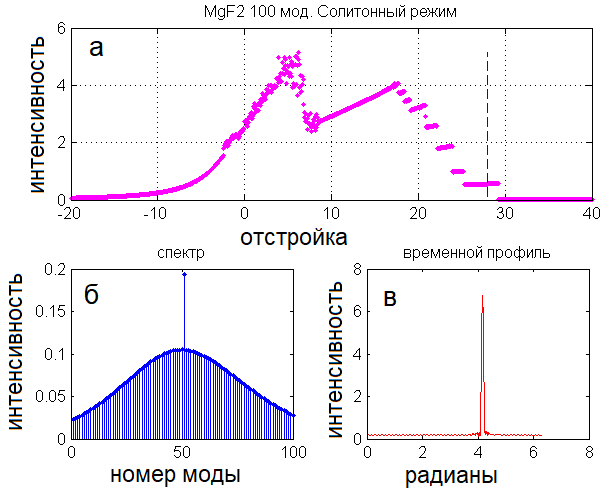
\includegraphics[width = 0.9\textwidth]{mgf2_100modes_aftoreferat}
  \setlength{\belowcaptionskip}{1pt} 
  \caption{Моделирование динамики генерации оптической частотной гребенки для 100 мод в резонаторе из MgF$_2$. Лазер накачки перестраивается по частоте линейно во времени. (а) Зависимость интенсивности суммарного поля внутри резонатора от отстройки частоты лазера, видны характерные ступеньки, соответствующие солитонному режиму. (б) спектр и (в) соответствующий ему временной профиль солитона на указанной вертикальном пунктиром отстройке.}
  \label{100modes}
\end{figure}

В п. 2.4 и 2.5 с помощью численного моделирования динамики оптических гребенок в микрорезонаторах с нормальной дисперсией групповой скорости резонатора, было найдено два новых метода генерации темных солитоноподобных структур (рис. \ref{platicons}): 1) метод, основанный на локальном изменении дисперсионного закона вблизи моды накачки; 2) метод, основанный на использовании двухчастотной или амплитудно-модулированной накачки с частотой модуляции кратной области свободной дисперсии резонатора. В обоих случаях были исследованы области существования и мягкого возбуждения оптических гребенок, определены зависимости от величины дисперсии, мощности накачки, глубины модуляции или величины сдвига моды накачки по частоте. Показано значительное увеличение суммарной мощности оптической гребенки в режиме нормальной дисперсии по сравнению с гребенками, получаемыми при аномальной дисперсии в микрорезонаторе.

\begin{figure}[!htb]
  \centering
  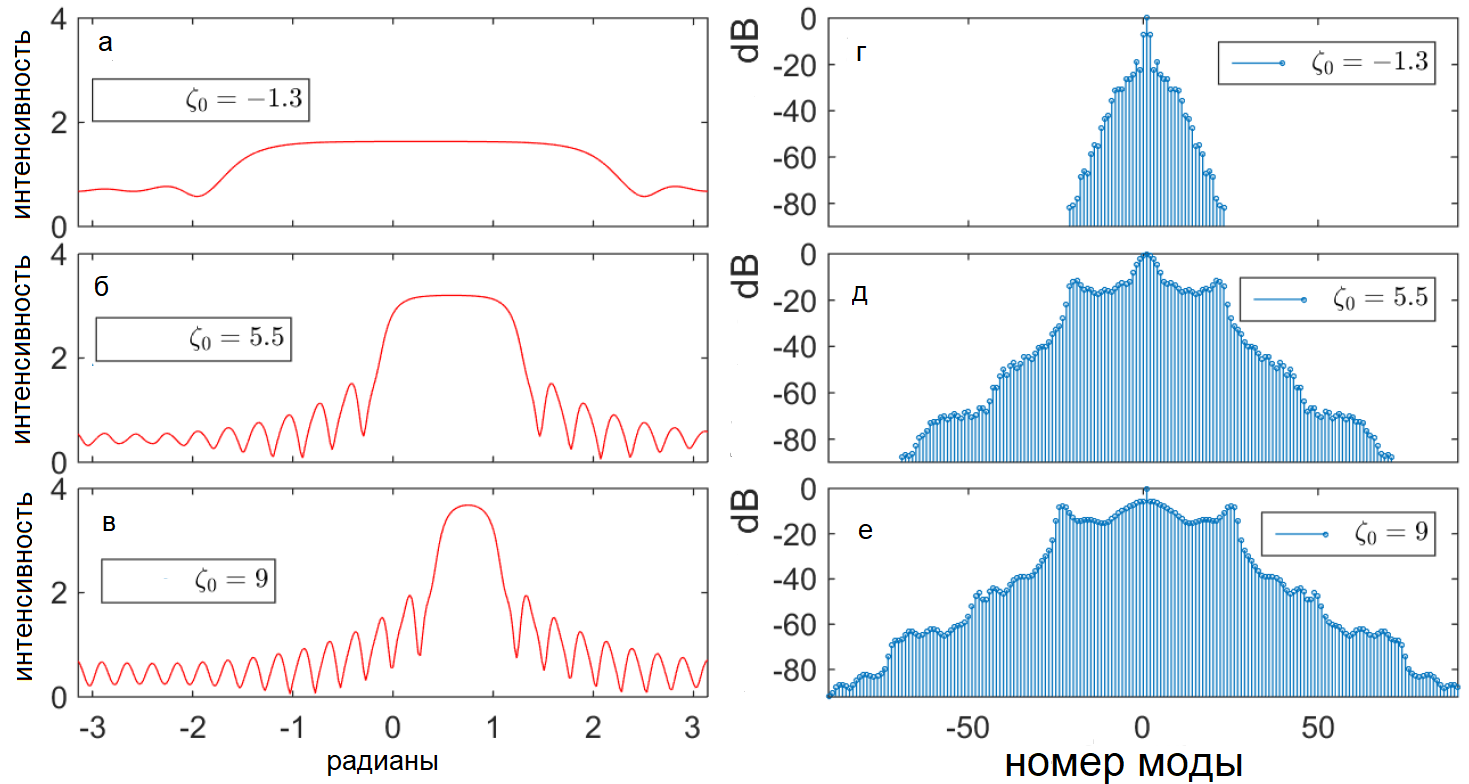
\includegraphics[width = 0.9\textwidth,height=0.4\textheight]{platicons_aftoreferat}
  \setlength{\belowcaptionskip}{1pt} 
  \caption{(а-в) Характерные профили поля внутри резонатора с нормальной дисперсией и (г-е) спектры темных солитоноподобных структур для различных значений отстройки частоты лазера ($\zeta_0$), получающиеся при локальном изменении дисперсионного закона вблизи моды накачки.}
  \label{platicons}
\end{figure}

Результаты главы 2 были опубликованы в статьях с номерами A1,A2,A3,A5 из списка публикаций.

\underline{\textbf{Третья глава}} посвящена экспериментальному исследованию методов генерации оптических частотных гребенок и солитонов в кристаллических микрорезонаторах и изучению их свойств.

В п. 3.1 разработана методика изготовления кристаллических микрорезонаторов методом алмазного точения с последующей полировкой алмазными суспензиями. Даны практические замечания по воспроизводимому изготовлению кристаллических микрорезонаторов заданной геометрии и высокой добротности. В ходе работы были изготовлены резонаторы с добротностью не менее $10^8$ из кристаллических материалов MgF$_2$, BaF$_2$, CaF$_2$, LiNbO$_3$, LiF, YLiF:Yb и с добротностью не менее $10^7$ из материалов: LiTaO$_3$, SiO$_2$, TGG, YLiF:Tm. Методика позволяет воспроизводимо изготавливать микрорезонаторы с заданной геометрией с точностью по диаметру до 1 мкм. Минимальный диаметр изготовленных резонаторов составил 100 мкм, максимальный 16 мм. Были успешно изготовлены резонаторы с микровыступами, в которых оптическое поле было локализовано в прямоугольном выступе на образующей цилиндра размером 5 на 10 мкм (см. рис. \ref{cavity_polished}).

\begin{figure}[!htb]
  \begin{minipage}{0.32\linewidth}\centering
    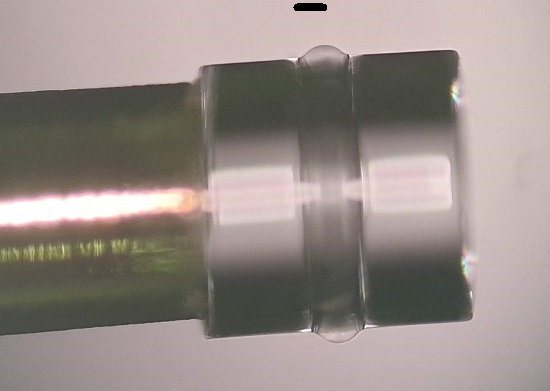
\includegraphics[width=1\linewidth]{caity1mm_polished}
  \end{minipage}
  \hfill
  \begin{minipage}{0.32\linewidth}\centering
    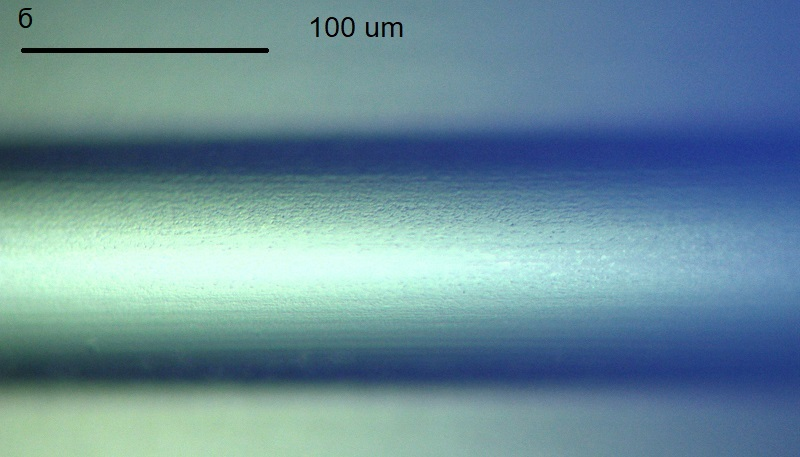
\includegraphics[width=1\linewidth]{protrusion_unpolished}
  \end{minipage}
  \hfill
  \begin{minipage}{0.32\linewidth}\centering
    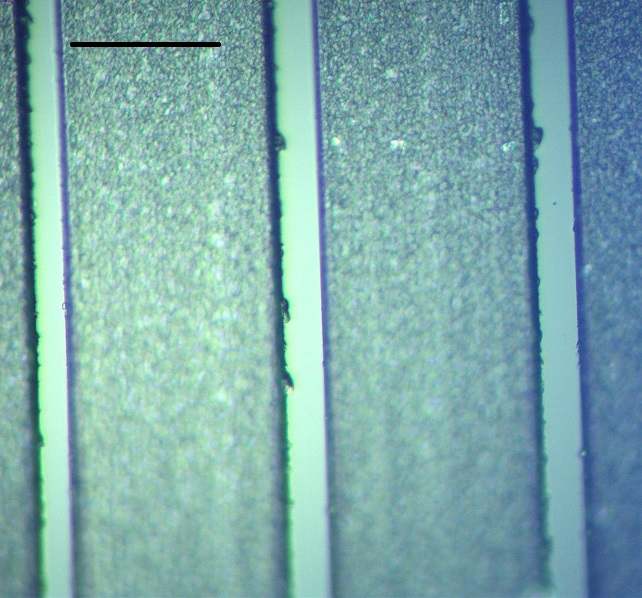
\includegraphics[width=1\linewidth]{protrsuion_rect}
  \end{minipage}
  \setlength{\belowcaptionskip}{1pt} 
  \caption{(а) фото отполированного резонатора диаметром 1 мм на латунной подставке. (б) фото поверхности резонатора из MgF$_2$ сразу после точения, в котором достигается добротность $10^6$. (в) фрагмент поверхности резонатора с прямоугольными выступами размером 5 на 20, 25 мкм.}
  \label{cavity_polished}
\end{figure}

В п. 3.2.1 дано описание экспериментальной установки, использующейся в большинстве экспериментов. Экспериментально продемонстрирована генерация некогеренных оптических частотных гребенок с шириной спектра до 300 нм в резонаторах из MgF$_2$. Продемонстрирован солитонный режим генерации в резонаторах из MgF$_2$ различного диаметра, с шириной спектра солитона до 120 нм при накачке на 1550 нм (см. рис \ref{clean_27GHz_single_soliton}). Измерен узкий сигнал биений (меньше 1 кГц) на частоте повторения солитона для различных микрорезонаторов. Показан метод контроля величины текущей отстройки частоты лазера накачки от собственной частоты моды резонатора с помощью анализатора цепей (панорамного индикатора) и фазовой модуляции лазера накачки с линейно изменяющейся частотой. Этот метод также позволяет определить наличие солитонного режима и количество распространяющихся солитонов в резонаторе без использования оптического спектроанализатора. Далее продемонстрирован метод стабилизации отстройки частоты лазера от моды резонатора с помощью схемы Паунда-Древера-Холла (PDH), показан вид сигнала ошибки, описан метод подбора оптимальных параметров для PID контроллера. Была измерена спектральная плотность мощности фазового шума сигнала биений на частоте повторения солитона со значениями -70 дБн/Гц на отстройке 1 кГц, -97 дБн/Гц на отстройке 10 кГц, для накачки резонатора использовался волоконный лазер с мгновенной шириной линии около 1 кГц. Отдельно было проведено сравнение генерации солитонов в микрорезонаторе в режиме затягивания многочастотного мощного диодного лазера на высокодобротную моду микрорезонатора из нелинейного материала MgF$_2$ и с накачкой перестраиваемым одночастотным волоконным лазером с усилителем. Показано, что обоими методами солитоны могут быть возбуждены на одном и том же семействе мод резонатора.

\begin{figure}[!htb]
  \begin{minipage}{0.49\linewidth}\centering
    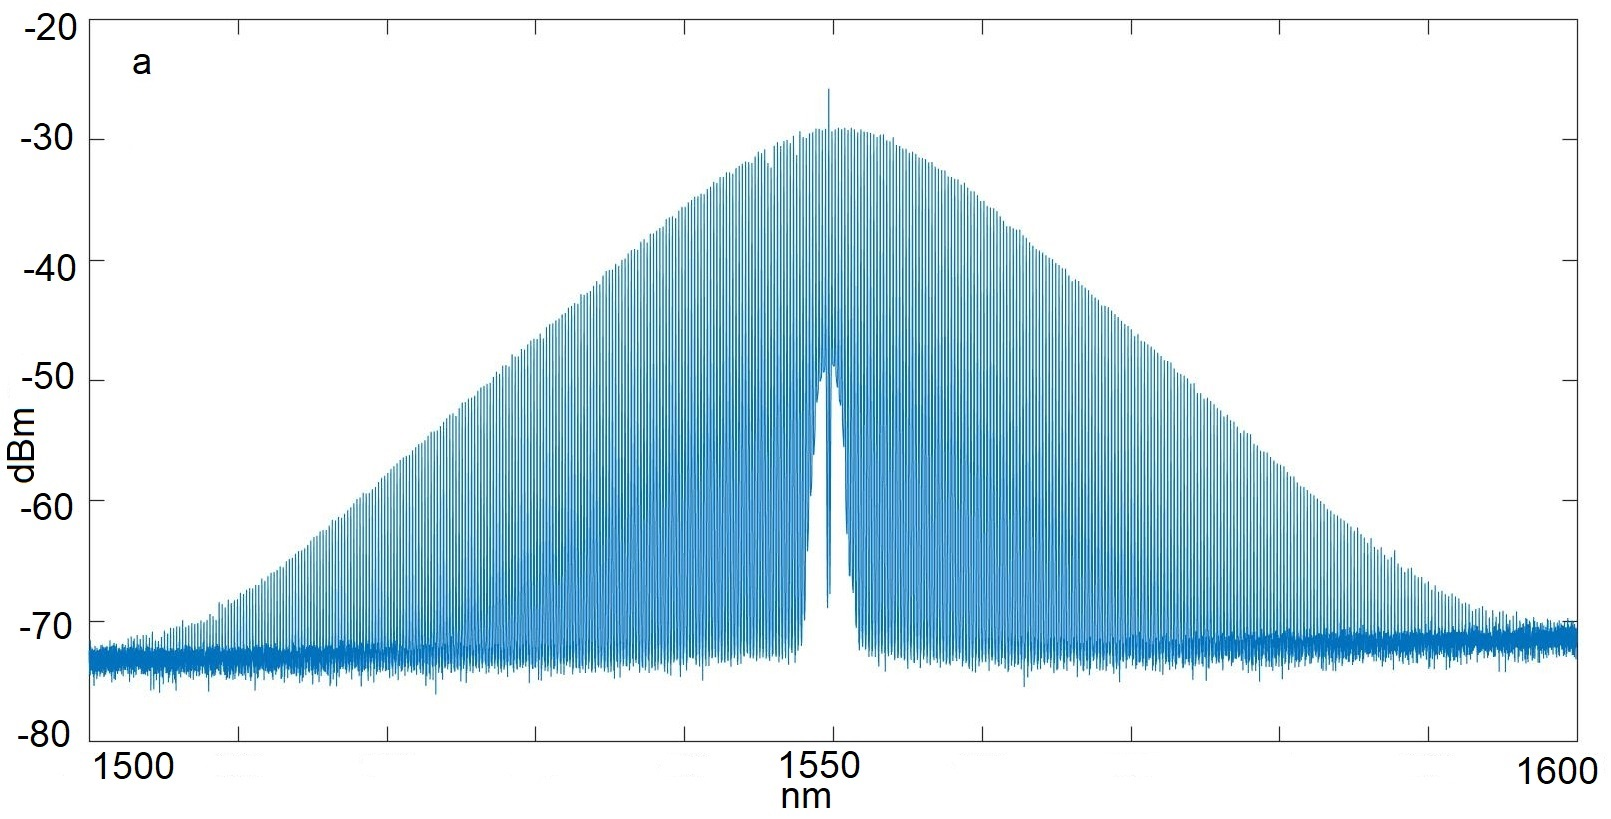
\includegraphics[width=1\linewidth]{clean_27GHz_single_soliton}
  \end{minipage}
  \hfill
  \begin{minipage}{0.49\linewidth}\centering
    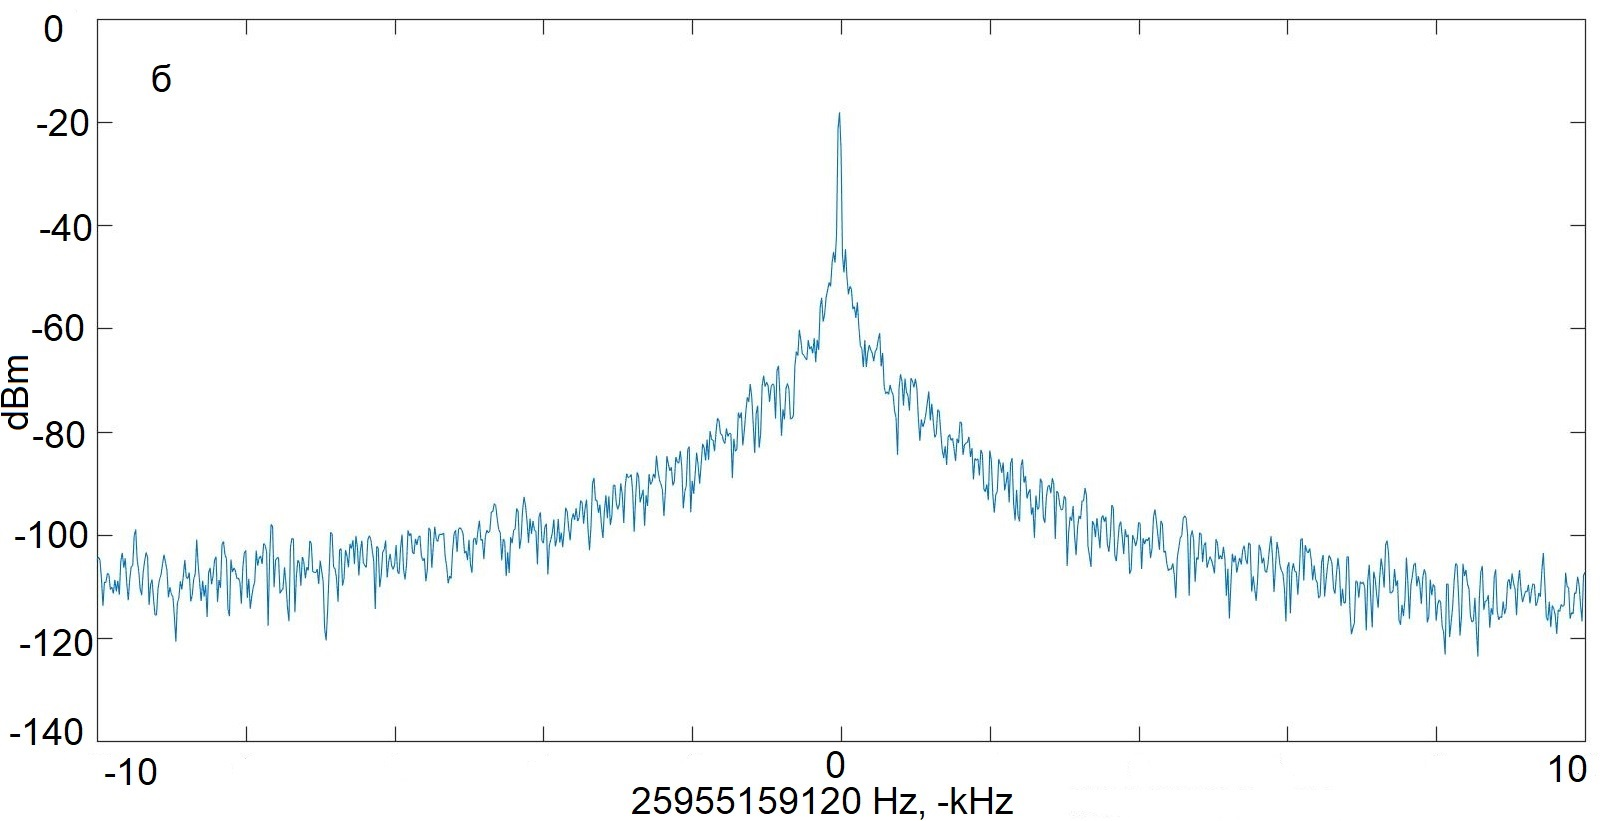
\includegraphics[width=1\linewidth]{26G_soliton_beat2_aftoreferat}
  \end{minipage}
  \setlength{\belowcaptionskip}{1pt} 
  \caption{(а) оптический спектр односолитонного режима, полученный в резонаторе диаметром 2.4 мм. (б) узкий сигнал биений на частоте повторения солитона 25.95 ГГц, ширина сигнала 100 Гц.}
  \label{clean_27GHz_single_soliton}
\end{figure}

В п. 3.2.2 показан метод достижения односолитонного режима с помощью фазовой или амплитудной модуляции лазера накачки на частоте повторения солитона. С помощью численного моделирования показано, что статистика генерации многосолитонных режимов значительно изменяется при включении слабой резонансной модуляции на частоте строго равной 1 области свободной дисперсии резонатора. Для фазовой модуляции возможны два равновероятных сценария: возбуждение односолитонного режима или отсутствие генерации солитонов. Показано, что важным фактором, увеличивающем вероятность односолитонного режима, является уменьшение скорости сканирования частоты лазера. Экспериментально показано, как модуляция накачки радикально меняет распределение вероятностей для числа генерируемых солитонов, и определены условия, при которых односолитонный режим становится достижимым и наиболее вероятным.

В п. 3.2.3 проведено исследование зависимости свойств солитонов от отстройки частоты лазера накачки. Ключевым параметром, описывающим динамику частотных гребенок и солитонов в микрорезонаторах является отстройка частоты лазера накачки от частоты резонанса. Из приближенного решения стационарного уравнения НУШ видно, что ширина гребенки пропорциональна квадратному корню из отстройки. При увеличении отстройки лазера мощность солитона растет, а длительность уменьшается (см. рис. \ref{detuning_dependant}), при этом незначительно растет частота повторения солитонов из-за сдвига его спектрального максимума, вызванного более сильным эффектом нормального расщепления мод. Величина отстройки также ограничивает максимально допустимое число солитонов в мультисолитонном режиме, которые могут распространяться без взаимодействия.

\begin{figure}[!htb]
  \begin{minipage}{0.49\linewidth}\centering
    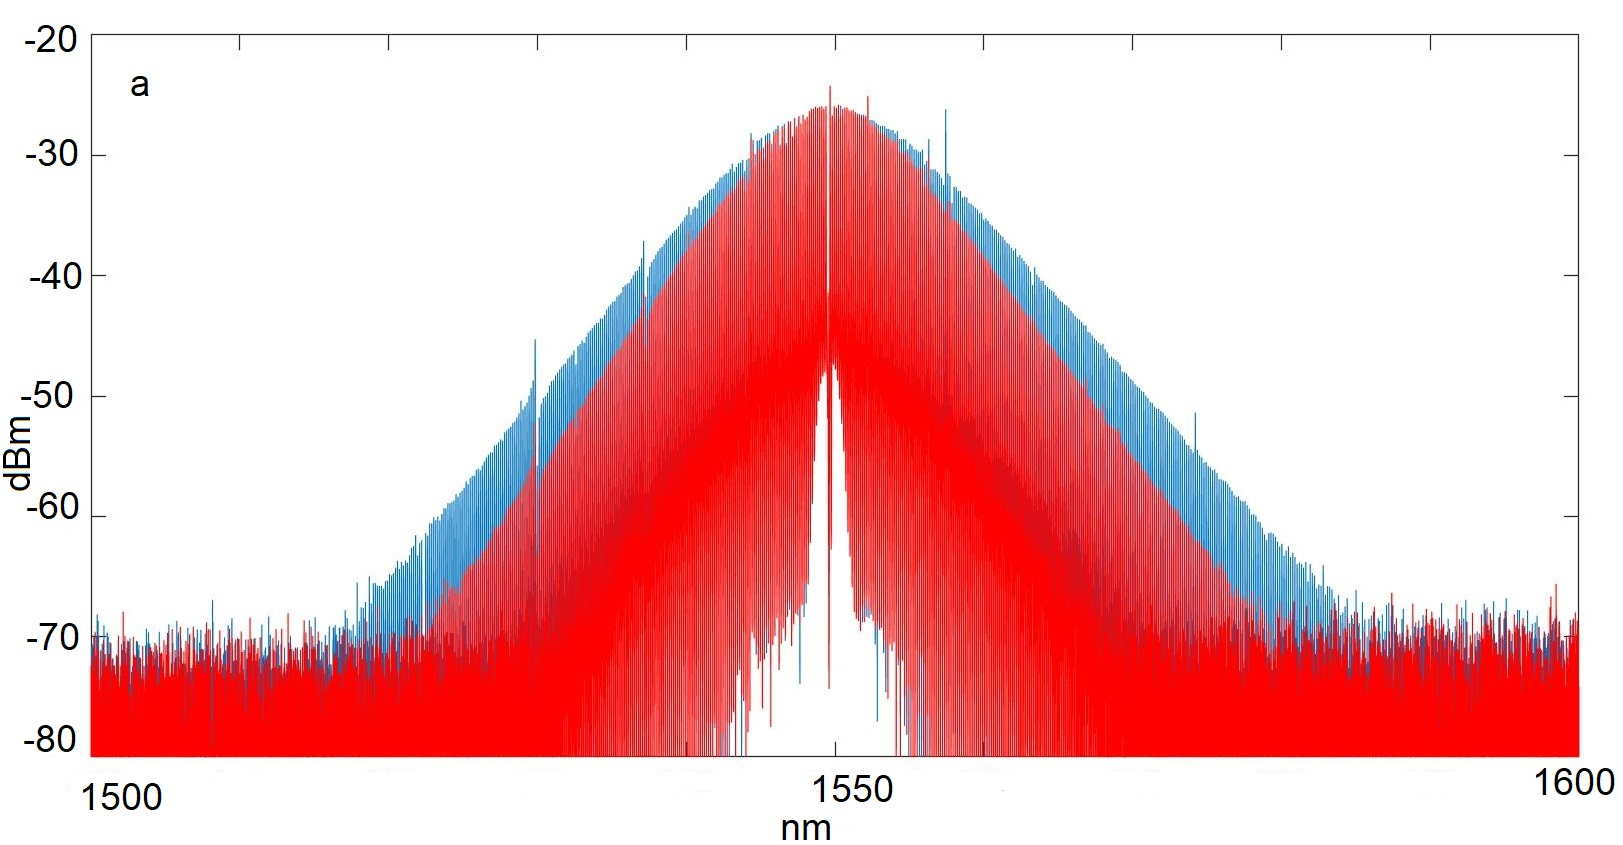
\includegraphics[width=1\linewidth]{soliton_span_vs_detuning_2_4MHz_aftoreferat}
  \end{minipage}
  \hfill
  \begin{minipage}{0.49\linewidth}\centering
    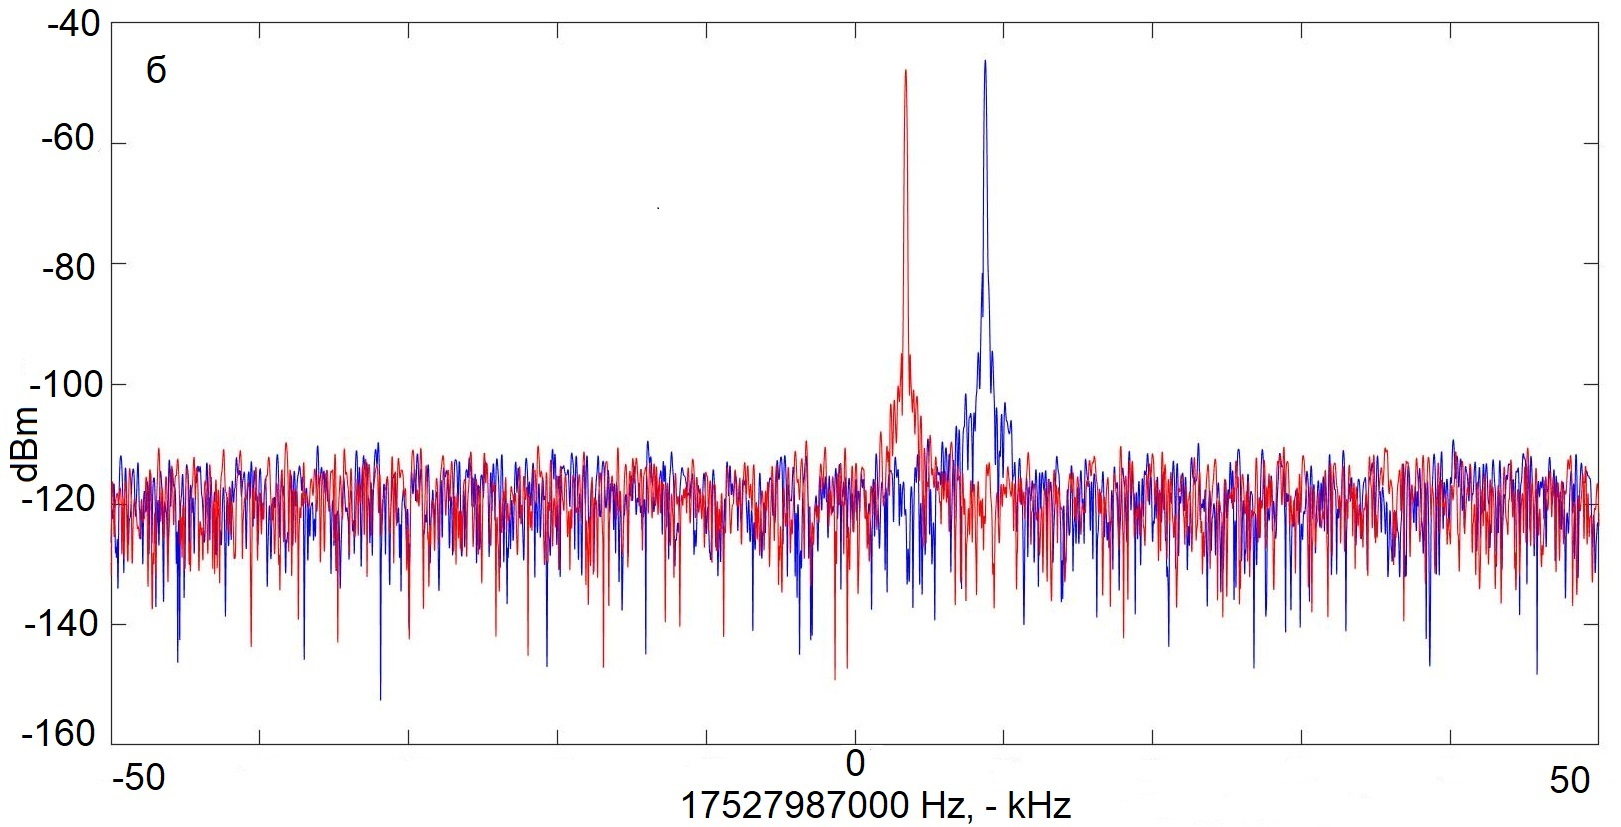
\includegraphics[width=1\linewidth]{reprates_vs_detuning_2_4MHz_aftoreferat}
  \end{minipage}
  \setlength{\belowcaptionskip}{1pt} 
  \caption{(а) оптические спектры односолитонных режимов, возбужденных на одной моде при разных отстройках частоты лазера накачки (красным - отстройка 2.5 МГц, синим - 4 МГц). (б) соответствующие сигналы биений на частоте повторения солитона, виден сдвиг частоты на 5 кГц при увеличении отстройки.}
  \label{detuning_dependant}
\end{figure}

В п. 3.2.4 показано экспериментально (см. рис. \ref{rep_rate_locking}), что при фазовой или амплитудной модуляции лазера накачки строго на частоте повторения солитона, возможно захватывание частоты повторения солитона частотой модуляции (диапазон захватывания около 1 кГц), т.ч. стабильность частоты повторения солитона на больших временах определяется стабильностью задающего генератора.

\begin{figure}[!htb]
  \centering
  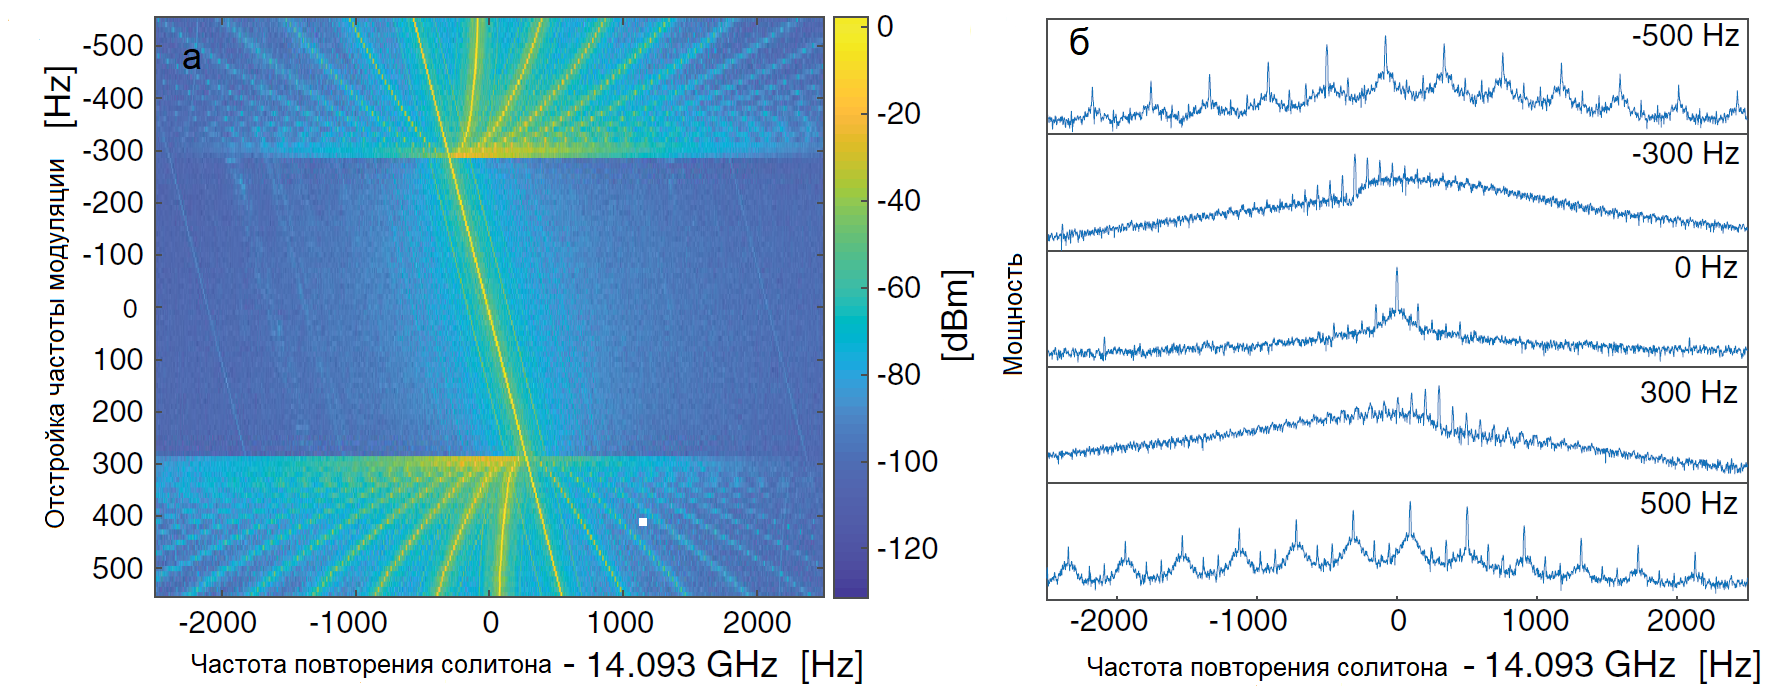
\includegraphics[width=0.99\linewidth]{rep_rate_locking}
  \setlength{\belowcaptionskip}{1pt} 
  \caption{(а) спектрограмма эффекта захватывания частоты повторения солитона на линейно перестраиваемую частоту фазовой модуляции лазера накачки, видна область затягивания шириной 600 Гц, (б) спектр сигнала, полученный на быстродействующем фотодетекторе в режиме без захватывания (-500 Гц) и с захватыванием (0 Гц).}
  \label{rep_rate_locking}
\end{figure}

В п. 3.3 представлены результаты экспериментального наблюдения термооптических осцилляций в микрорезонаторе из BaF$_2$ при накачке лазером мощностью 25 мВт. В резонаторах из BaF$_2$ диаметром 3.9 мм экспериментально наблюдался эффект вынужденного рассеяния Мандельштама-Бриллюэна при накачке на длине волны 1550 нм, измерена частота сдвига Мандельштама-Бриллюэна в 8.27 ГГц и ширина соответствующих сигналов биений. В микрорезонаторе диаметром 400 мкм из BaF$_2$ экспериментально продемонстрирована каскадная генерация нескольких линий оптической частотной гребенки на значительном удалении от линии накачки и одновременное вынужденное комбинационное рассеяние на длине волны 1615 нм, что соответствует табличному значению для рамановского сдвига в материале.

Результаты главы 3 были опубликованы в статьях с номерами A4,A6,A8,A10,A11 из списка публикаций.
%Можно сослаться на свои работы в автореферате. Для этого в файле
%\verb!Synopsis/setup.tex! необходимо присвоить положительное значение
%счётчику \verb!\setcounter{usefootcite}{1}!. В таком случае ссылки на
%работы других авторов будут подстрочными.
%\ifnumgreater{\value{usefootcite}}{0}{
%Изложенные в третьей главе результаты опубликованы в~\cite{vakbib1, vakbib2}.
%}{}
%Использование подстрочных ссылок внутри таблиц может вызывать проблемы.

В \underline{\textbf{четвертой главе}} приведены методы генерации двойных оптических гребенок и солитонов в кристаллических микрорезонаторах.

В п. 4.1 экспериментально показана одновременная генерация двух солитонных оптических гребенок в двух различных резонаторах при накачке двумя независимыми лазерами (см. рис. \ref{ris:image1}). Для генерации нескольких солитонных оптических гребенок с практически идентичными частотами повторения была разработана структура с несколькими резонаторами одинаковой формы, выточенными на одном кристаллическом цилиндре из MgF$_2$. В результате финальной полировки разница в ОСД между несколькими резонаторами была не более 10 МГц, что соответствует разнице в радиусах резонаторов в 0.5 мкм при условии возбуждении одного семейства мод в обоих резонаторах. Солитоны были получены последовательно в трех из пяти резонаторах на одном цилиндре. При одновременном возбуждении оптические спектры мультисолитонных состояний в обоих резонаторах содержат более 300 линий, разделенных по $12.1$ ГГц и покрывает 35 нм около центральной частоты 1554 нм. Результирующий сигнал биений на фотодетекторе от двух оптических гребенок отображает двойную оптическую гребенку в радиодиапазон, имеет общую ширину 300 МГц с центром на 1.07 ГГц и содержит около 150 линий, разделенных на $1.62$ МГц, каждая шириной 200 кГц и имеет огибающую, совпадающую с оптическими профилями двух солитонов.

\begin{figure}[!htb]
\begin{minipage}{1\linewidth}
\center{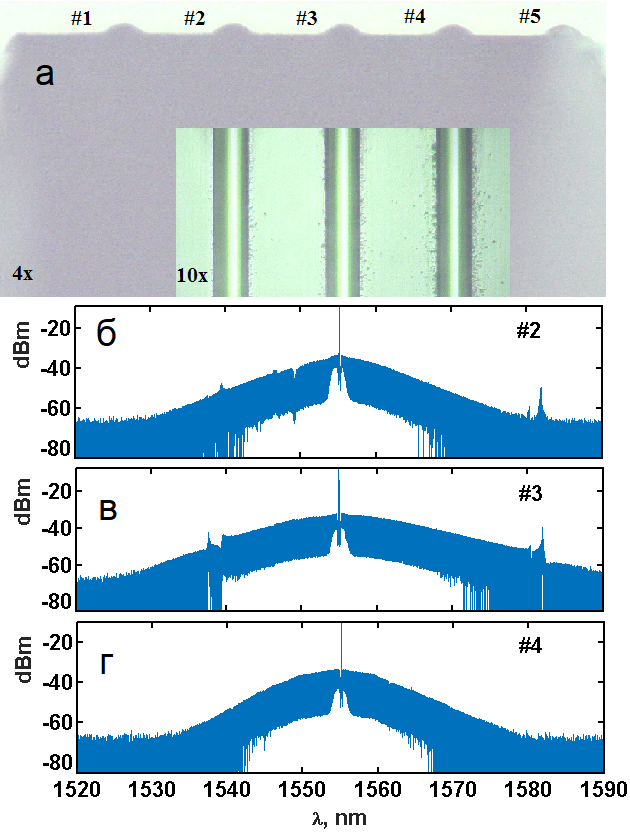
\includegraphics[width=0.5\linewidth]{dual_cavity_aftoreferat}}
\end{minipage}
\setlength{\belowcaptionskip}{4pt} 
\caption{(a): Фото стэка резонаторов на одном кристаллическом цилиндре с диаметром 5.68 мм. Вставка показывает 3 отполированных резонатора, в которых наблюдались солитоны; (б-г): оптический спектр солитонов, генерируемых в 3 различных резонаторах. Солитонные керровские частотные гребенки имеют ширину $30 - 65$ нм с расстоянием между линиями 12.1 ГГц.}
\label{ris:image1}
\end{figure}

В п. 4.2 экспериментально показана одновременная генерация двух солитонных оптических гребенок в одном резонаторе на разных семействах мод, распространяющихся в одном направлении (см. рис. \ref{Figure1_V1_c}), при накачке мощным перестраиваемым лазером и одной боковой линией амплитудной модуляции лазера. На рис. \ref{Co_Scheme_results} показаны оптические спектры одновременно двух солитонов на разных семействах мод с разницей по частоте накачки $4.28$ ГГц. Разница в частотах повторения солитонов составила $655$ кГц (частота повторения $12.4$ ГГц). Ширина индивидуальных линий результирующей СВЧ гребенки менее 100 Гц, что говорит о высокой взаимной когерентности двух солитонов, хотя вся система не стабилизирована (частота повторения солитонов и лазер накачки не привязаны ни к каким эталонам). Отображение оптического спектра двойной гребенки на СВЧ спектр взаимно однозначно, 200 МГц радио спектра отображаются на 3 ТГц оптического диапазона без каких-либо наложений. Экспериментально показано, что хотя солитоны распространяются в различных пространственных семействах мод, они могут эффективно взаимодействовать между собой через четырехволновое взаимодействие, и могут быть модулированными на частоте, кратной разности частот повторений солитонов.

\begin{figure}[!htb]
\begin{minipage}{1\linewidth}
\center{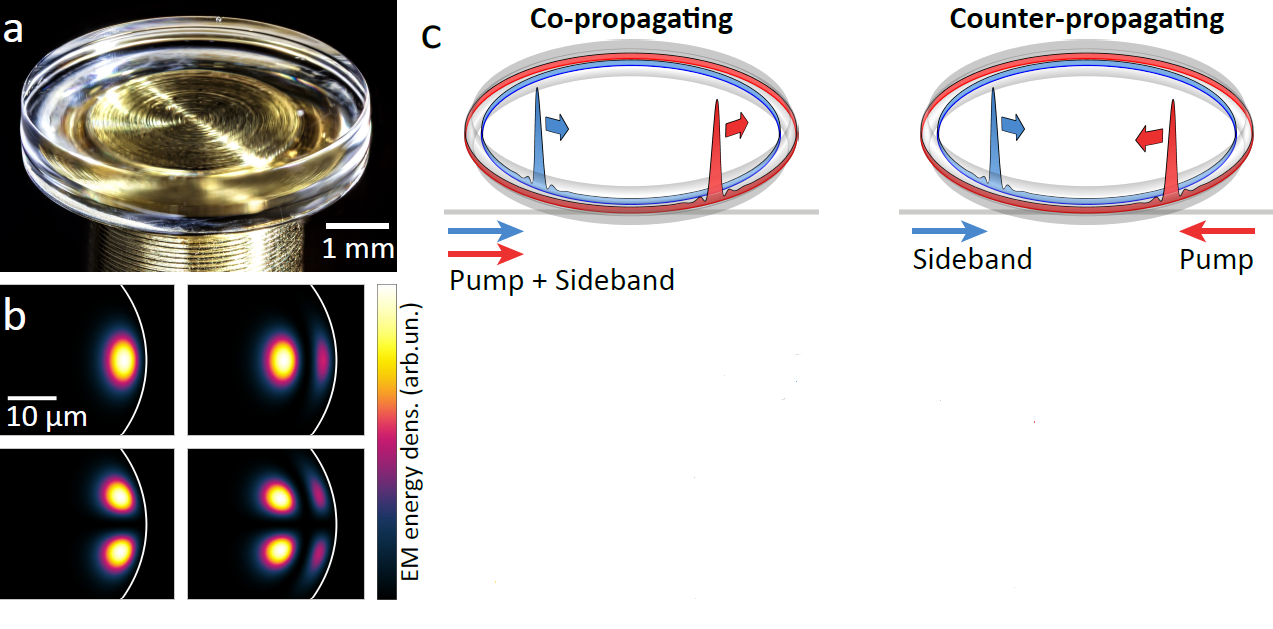
\includegraphics[width=0.75\linewidth]{fig1_scheme_general}}
\end{minipage}
\setlength{\belowcaptionskip}{4pt} 
\caption{(а) Фотография многомодового резонатора MgF$_2$ диаметром 5.5 мм; (b) примеры численного моделирования различных семейств мод и распределения электрического поля внутри МШГ; (с) схема возбуждения солитонов с распространением в одном или противоположных направлениях.}
\label{Figure1_V1_c}
\end{figure}

\begin{figure}[!htb]
\begin{minipage}{1\linewidth}
\center{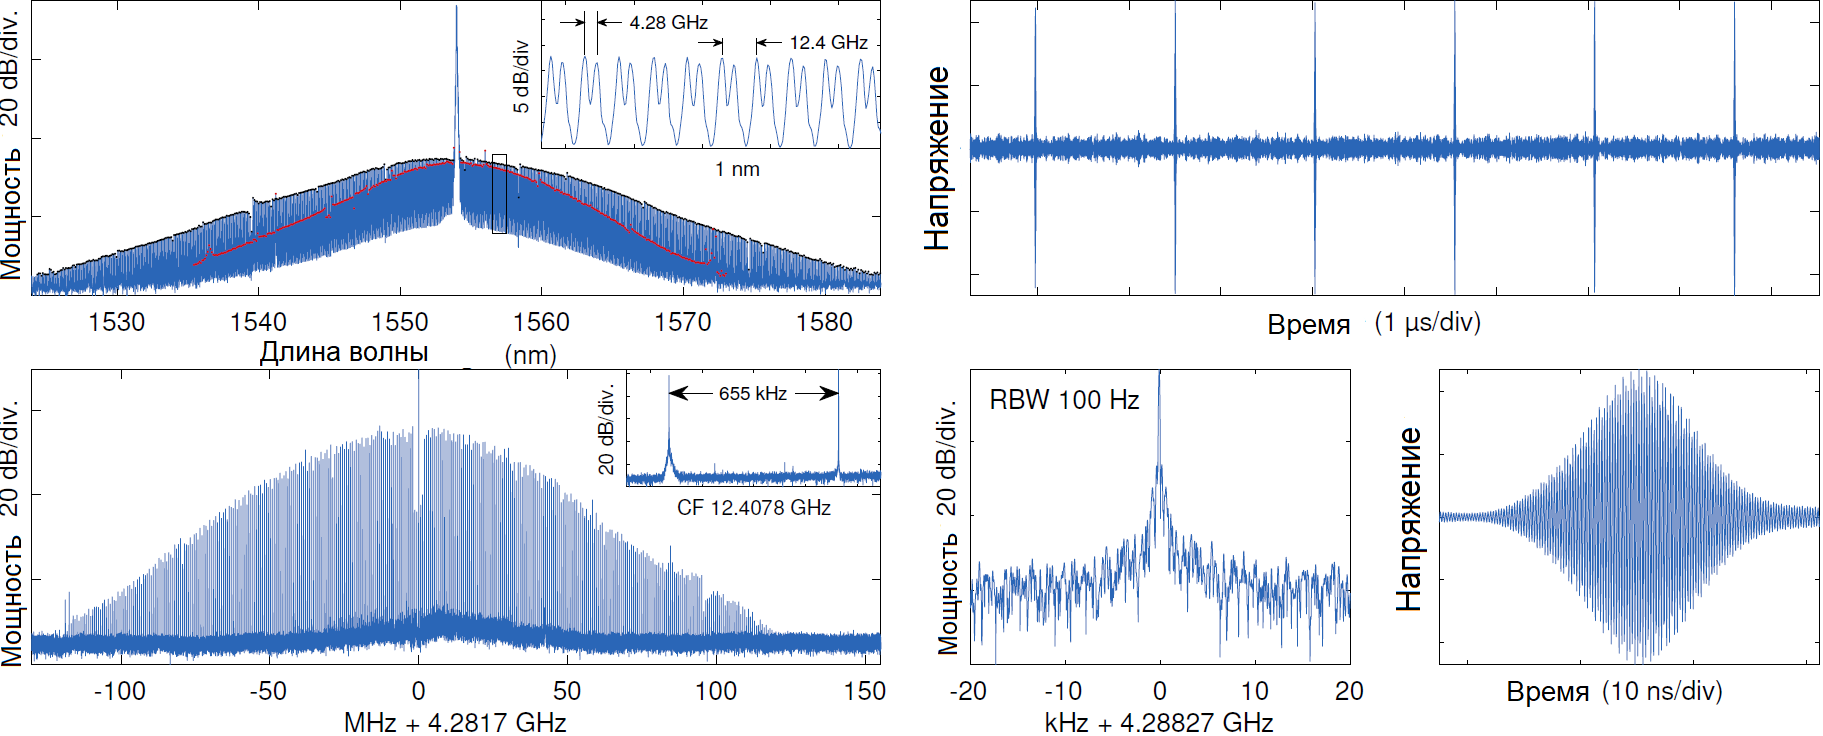
\includegraphics[width=1\linewidth]{Co_Scheme_results}}
\end{minipage}
\setlength{\belowcaptionskip}{4pt} 
\caption{Экспериментальные результаты одновременного возбуждения односолитонных режимов на двух разных семействах мод в 1 микрорезонаторе. (а) суммарный оптический спектр односолитонных режимов, красной линией помечена огибающая второго солитона, на вставке представлены отдельные оптические линии двух солитонов. ОСД резонатора 12.4 ГГц, расстояние между несущими 4.28 ГГц. (б) результирующий сигнал биений двух солитонов на быстром фотодиоде - СВЧ гребенка с расстоянием между линиями 655 кГц, которое соответствует разнице между ОСД семейств мод, на вставке изображены сигналы частот повторения двух солитонов, (в) сигнал последовательности результирующих СВЧ импульсов, снятый быстрым осциллографом, (г) одиночная нецентральная линия СВЧ гребенки шириной менее 100 Гц, (д) сигнал одиночного СВЧ импульса.}
\label{Co_Scheme_results}
\end{figure}

В п. 4.3 экспериментально показана одновременная генерация двух солитонных оптических гребенок в одном резонаторе на разных семействах мод, распространяющихся в противоположных направлениях (см. рис. \ref{Figure1_V1_c}), при накачке мощным перестраиваемым лазером и одной боковой линией амплитудной модуляции лазера. Были использованы моды из пары семейств с разницей в собственных частотах $2.75$ ГГц и разницей в частотах повторения $371$ кГц, оптические спектры односолитонных режимов даны на рис. \ref{counter_prop_results}. Мощность каждого солитона после подавления накачки около 400 мкВт. Соответствующая результирующая СВЧ гребенка имела тот же уровень стабильности, что и в схеме с распространением в одном направлении, с шириной индивидуальной линии около 500 Гц. Показано основное преимущество схемы - отсутствие кроссмодуляции между солитонами, и возможность их разделить в пространстве и использовать отдельно. Далее продемонстрировано применение метода двойной оптической гребенки для прямой спектроскопии поглощения веществ, измерены оптические линии поглощения шириной порядка 100 ГГц с разрешением, определяющимся ОСД резонатора 12.4 ГГц.

\begin{figure}[!htb]
\begin{minipage}{1\linewidth}
\center{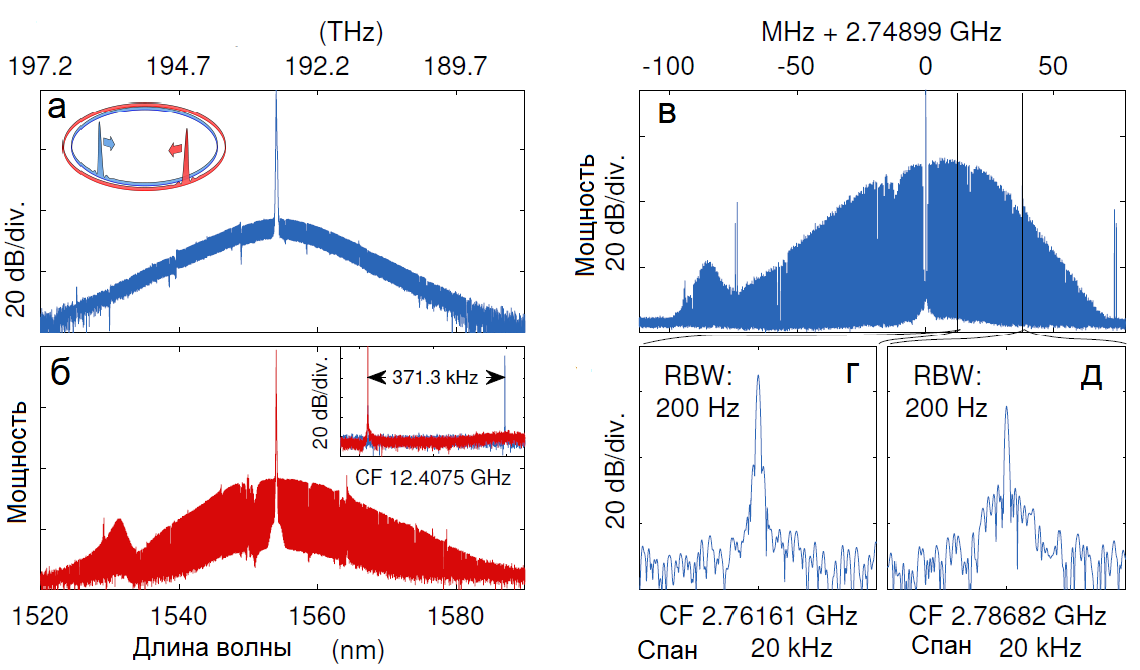
\includegraphics[width=1\linewidth]{counter_prop_results}}
\end{minipage}
\setlength{\belowcaptionskip}{4pt} 
\caption{Экспериментальные результаты одновременного возбуждения солитонов в противоположных направлениях в 1 резонаторе на разных семействах мод. (а,б) Оптические спектры односолитонных режимов, полученных на разных семействах. На вставке показаны наложенные друг на друга сигналы биений на частоте повторения солитонов. Разница в частотах повторений составила 371 кГц. (в) Результирующая СВЧ гребенка, получаемая на фотодетекторе при совмещении солитонов, распространяющихся в противоположном направлении, центральная частота совпадает с частотой модуляции 2.748 ГГц, расстояние между линиями 371 кГц. (г,д) Ширина индивидуальных линий СВЧ гребенки порядка 500 Гц.}
\label{counter_prop_results}
\end{figure}

В п. 4.4 описывается экспериментально продемонстрированая одновременная генерация солитонных оптических гребенок в одном резонаторе на одном семействе мод в противоположных направлениях. Показано, что предложенный в п. 4.3 метод генерации солитонов в одном резонаторе в противоположных направлениях применим не только при накачке разных семейств мод, но возможен и на одном семействе мод, для этого на амплитудный модулятор подается частота не выше максимальной отстройки, при которой существует солитон. Так как частота повторения солитонов зависит от отстройки частоты накачки, то при небольшом сдвиге накачки в прямом и обратном направлениях возможно образование результирующей СВЧ гребенки. Найдено пороговое значение отстройки (2 МГц), меньше которой частоты повторения солитонов строго совпадают и двойная гребенка не наблюдается. Экспериментально обнаружено, что частоты повторений солитонов могут совпасть и при таком значении отстройки, когда проявляются сильные эффекты нормального расщепления мод.

Результаты главы 4 были опубликованы в статьях с номерами A7,A9 из списка публикаций.

В \underline{\textbf{заключении}} приведены основные результаты работы, которые заключаются в следующем:
%% Согласно ГОСТ Р 7.0.11-2011:
%% 5.3.3 В заключении диссертации излагают итоги выполненного исследования, рекомендации, перспективы дальнейшей разработки темы.
%% 9.2.3 В заключении автореферата диссертации излагают итоги данного исследования, рекомендации и перспективы дальнейшей разработки темы.
\begin{enumerate}
  \item Численные исследования модели уравнений связанных мод показали, что в высокодобротных микрорезонаторах возможна генерация оптических временных солитонов, были изучены диапазоны параметров и условия, влияющие на их эффективную генерацию.
  \item Математическое моделирование показало, что при нормальной ДГС резонатора возможна генерация темных солитоноподобных структур при условии наличия изменения в законе дисперсии или при использовании двухчастотной или амплитудно-модулированной накачки. 
  \item Для выполнения экспериментальных исследований была разработана методика изготовления кристаллических микрорезонаторов методом алмазного точения и полировки алмазными суспензиями.
  \item Экспериментально была продемонстрирована генерация оптических солитонов в резонаторах из $MgF_2$ с ОСД от $8.5$ до $27$ ГГц. При активной стабилизации температуры и отстройки частоты лазера накачки солитон существовал длительное время, достаточное для экспериментальной демонстрации применений.
  \item Впервые продемонстрирована возможность одновременнной генерации солитонов в идентичных микрорезонаторах, расположенных на одном кристаллическом цилиндре.
  \item Впервые продемонстрирована возможность одновременнной генерации солитонов в одном резонаторе на разных семействах пространственных мод, распространяющихся как в одном, так и в противоположных направлениях.
  \item Для дальнейших исследований в данной области важной задачей является экспериментальная демонстрация широких, октавных гребенок в солитонном режиме, гребенок в кристаллических резонаторах с нормальной дисперсией. Из новых практических применений возможна демонстрация фотонного АЦП с использованием двойных оптических гребенок, демонстрация калибровки астрономических эшелле спектрометров.
\end{enumerate}



\section*{Список публикаций автора по теме диссертации, индексируемых в базах данных Web of Science и Scopus:}

\begin{enumerate}[label=\sbscript{A}{{\arabic*}}.]
  \item Herr T., Brasch V., Jost J.D., Mirgorodskiy I., Lihachev G., Gorodetsky M.L., Kippenberg T.J. Mode spectrum and temporal soliton formation in optical microresonators // Phys. Rev. Lett. — 2014. — Vol. 113. — P. 123901
  \item Lobanov V.E., Lihachev G., Kippenberg T.J., Gorodetsky M.L. Frequency combs and platicons in optical microresonators with normal GVD // Opt. Express. — 2015. — Vol. 23. — Pp. 7713–772
  \item V.E. Lobanov, G. Lihachev, M.L. Gorodetsky. Generation of platicons and frequency combs in optical microresonators with normal GVD by modulated pump // EPL. — 2015. — Vol. 112. — P. 54008.
  \item Lobanov V.E., Lihachev G.V., Pavlov N.G. et al. Harmonization of chaos into a soliton in Kerr frequency combs // Optics Express. — 2016. — Vol. 24, no. 24.— Pp. 27382–27394.
  \item Brasch V., Geiselmann M., Herr T., Lihachev G., Pfeiffer M.H.P, Gorodetsky M.L., Kippenberg T.J. Photonic chip based optical frequency comb using soliton induced Cherenkov radiation // Science. — 2016. — Vol. 351, no. 6271. — Pp. 357–360.
  \item Guo H., Karpov M., Lucas E., Kordts A., Pfeiffer M.H.P, Brasch V., Lihachev G., Lobanov V.E., Gorodetsky M.L., Kippenberg T.J. Universal dynamics and deterministic switching of dissipative Kerr solitons in optical microresonators // Nature Phys. — 2017. — Vol. 13, no. 1. — P. 94–102
  \item Pavlov N.G., Lihachev G., Koptyaev S. et al. Soliton dual frequency combs in crystalline microresonators // Optics Lett. — 2017. — Vol. 42, no. 3. — Pp. 514–517.
  \item M. Anderson, N. G. Pavlov, J. D. Jost, G. Lihachev, J. Liu, T. Morais, M. Zervas, M. L. Gorodetsky, T. J. Kippenberg. Highly efficient coupling of crystalline microresonators to integrated photonic waveguides // Opt. Lett. — 2018. — Vol. 43, no. 9. — Pp. 2106–2109
  \item E. Lucas, G. Lihachev, R. Bouchand et al. Spatial multiplexing of soliton microcombs // Nature Photonics. — 2018. — Vol. 12, no. 11. — Pp. 699–705.
  \item N. G. Pavlov, S. Koptyaev, G. V. Lihachev et al. Narrow-linewidth lasing and soliton Kerr microcombs with ordinary laser diodes // Nature Photonics. — 2018. — Vol. 12, no. 11. — Pp. 694–698
  \item W. Weng, E. Lucas, G. Lihachev et al.  Spectral Purification of Microwave Signals with Disciplined Dissipative Kerr Solitons // Phys. Rev. Lett. — 2019. — Vol. 122. — P. 013902
\end{enumerate}



%\newpage
%При использовании пакета \verb!biblatex! список публикаций автора по теме
%диссертации формируется в разделе <<\publications>>\ файла
%\verb!../common/characteristic.tex!  при помощи команды \verb!\nocite!

\ifdefmacro{\microtypesetup}{\microtypesetup{protrusion=false}}{} % не рекомендуется применять пакет микротипографики к автоматически генерируемому списку литературы
\ifnumequal{\value{bibliosel}}{0}{% Встроенная реализация с загрузкой файла через движок bibtex8
  %\renewcommand{\bibname}{\large \authorbibtitle}
  %\nocite{*}
  %\insertbiblioauthor           % Подключаем Bib-базы
  \insertbibliofull
  %\insertbiblioother   % !!! bibtex не умеет работать с несколькими библиографиями !!!
}{% Реализация пакетом biblatex через движок biber
  \ifnumgreater{\value{usefootcite}}{0}{
%  \nocite{*} % Невидимая цитата всех работ, позволит вывести все работы автора
  \insertbiblioauthorcited      % Вывод процитированных в автореферате работ автора
  }{
  \insertbiblioauthor           % Вывод всех работ автора
%  \insertbiblioauthorgrouped    % Вывод всех работ автора, сгруппированных по источникам
%  \insertbiblioauthorimportant  % Вывод наиболее значимых работ автора (определяется в файле characteristic во второй section)
  \insertbiblioother            % Вывод списка литературы, на которую ссылались в тексте автореферата
  }
}
\ifdefmacro{\microtypesetup}{\microtypesetup{protrusion=true}}{}

      % Содержание автореферата

%%% Выходные сведения типографии
\newpage\thispagestyle{empty}

\vspace*{0pt plus1fill}

\small
\begin{center}
    \textit{\thesisAuthor}
    \par\medskip
    
    \thesisTitle
    \par\medskip
    
    Автореф. дис. на соискание ученой степени \thesisDegreeShort
    \par\bigskip
    
    Подписано в печать \blank[\widthof{999}].\blank[\widthof{999}].\blank[\widthof{99999}].
    Заказ № \blank[\widthof{999999999999}]
    
    Формат 60\(\times\)90/16. Усл. печ. л. 1. Тираж 100 экз.
    %Это не совсем формат А5, но наиболее близкий, подробнее: http://ru.wikipedia.org/w/index.php?oldid=78976454
    
    Типография \blank[0.5\linewidth]
\end{center}
\cleardoublepage

\end{document}